%
% University of Fribourg
%
% Master Thesis Template
% Thomas Kolonko 13.04.2019
%

\documentclass[11pt,a4paper,twoside,hidelinks,openright]{rvsmaster}

\usepackage[latin1]{inputenc}
\usepackage{graphicx}
\usepackage{float}
\graphicspath{ {./images/} }
%%%%%%%%%%%%%%%%%%%%%%%%%%%%%%%%%%%%%%%%%%%%

\usepackage[a4paper,twoside]{geometry}

\sloppy

%% Additional packages
%%%%%%%%%%%%%%%%%%%%%%%%%%%%%%%%%%%%%%%


\usepackage{mathpazo}

% for source code highlighting
% \usepackage{listings}
% \lstloadlanguages{tcl, Perl}
% \lstset{language=tcl, commentstyle=\it, basicstyle=\tiny, keywordstyle=\bf, breaklines=true, frame=single}

% multiple figures with same general caption. FIGTOPCAP puts the subcaption on top of the figures
\usepackage[FIGTOPCAP]{subfigure}
\setcounter{lofdepth}{2}  

% offers more possibilities in captions
\usepackage{caption}


% Tool for handling the figure on multicolumns or multirows
\usepackage{multicol}
\usepackage{multirow}

% Main page with logos...
\usepackage{unifrmr}


% Fancy tables
\usepackage{booktabs}
\newcommand{\ra}[1]{\renewcommand{\arraystretch}{#1}}
\usepackage[font={small,it}]{caption} 
\captionsetup[table]{skip=10pt}
\usepackage{array}

\usepackage{listings}

\newcolumntype{L}[1]{>{\raggedright\arraybackslash}p{#1}}

% Commands for package caption
% - caption
\renewcommand{\captionfont}{\small}
\renewcommand{\captionlabelfont}{\bfseries}

% offers rotation of figures, ...
\usepackage{rotating}

% to support correct hyphenaten, add words with -
% \hyphenation{test-case}

% If a page has no content, make it an empty page (without page numbers ....)
\makeatletter
\def\cleardoublepage{\clearpage\if@twoside \ifodd\c@page\else
	\hbox{}
	\thispagestyle{empty}
	\newpage
\fi\fi}
\makeatother


% check whether we are running pdflatex
\newif\ifpdf
\ifx\pdfoutput\undefined
\pdffalse % we are not running pdflatex
\DeclareGraphicsExtensions{.eps}
\else
\pdfoutput=1 % we are running pdflatex
\pdfcompresslevel=9     % compression level for text and image;
\pdftrue
\DeclareGraphicsExtensions{.pdf,.png,.jpg}
\fi
\ifpdf
%to make table of contents and index appear in bookmarks
\usepackage{tocbibind}
%refs also as links
\usepackage[pdftex,plainpages=false]{hyperref}
%plainpages=false: enable links although page numbering is reset after title
%backref, pagebackref]{hyperref}
%\usepackage[pdftex]{color}
%\usepackage[pdftex]{thumbpdf}
\else
%url must be escaped. (this works fine in dvi)
\usepackage{url}
\fi


\author{Thomas Kolonko\thanks{\email{thomas.kolonko@students.unibe.ch}, HumanTech group, University of Fribourg}}
\title{Asbestos Detection in Microscopic Imaging}
\date{April 15, 2019} % Note: if this is left out, today's date will be used.

\begin{document}
\maketitle
\thispagestyle{empty}
\mbox{}

\newpage

\chapter*{Abstract}

Asbestos is a highly toxic silicate mineral that has been used widely in many products for its insulating, non-flammable and heat resistant properties. It may lead to chronic inflammation of the lungs and cancer when exposed to high concentrations. After the toxicity has become known, much effort was undertaken - and is up to this day - in removing asbestos from buildings, roofs and other materials used in industry and in the public. Asbestos detection is a manual, complex and time-intensive process, that requires a lot of experience from an expert in order to have consistent and correct results. In order to reduce manual labor and increase consistency in detection, machine learning models have been recently adopted to automate the detection process.

\vspace{5mm} %5mm vertical space

Convolutional Neural Networks have the property of automatically extracting feature mappings from the provided dataset and applying these feature mappings on the images in a spatial relevant manner. These feature mappings are adjusted with each iteration in order to represent the training data and thus minimizing the loss function. These properties make Convolutional Neural Networks a very good fit for the task of detecting asbestos fibers. Especially by reducing the needed knowledge about asbestos and experience acquired through years of working with asbestos which is one of the main prerequisites of a laboratory to be successful in the detection of asbestos fibers.

\vspace{5mm} %5mm vertical space

In this thesis, several state-of-the-art architectures are explained and compared against each other in regard of performance accuracy, size, and complexity. I will evaluate if transfer learning from the ImageNet dataset can be applied in this specific cross-domain task of asbestos fiber detection. in microscopic images. Data augmentation with different cropping methods will be implemented and compared with the goal of increasing the overall accuracy of the model. Since the dataset is quite small, with only about 2'000 images, several train and valuation datasets and their distribution are evaluated. The test set is fixed in the beginning and never altered. Another branch of investigation will be alterations to the current architectures like reducing the filters and fully connected layers in order to decrease complexity and increase interpretability through visualization. Also, adding new layers in order to allow the input image to be bigger, thus reducing problems that arise with cropping and re-sizing the original image are investigated.

\vspace{5mm} %5mm vertical space

I succeeded to show that transfer learning on ImageNet does indeed benefit the asbestos detection task on microscopic images for all used architectures. I show through visualizations that this is mostly due to the mid- and high-level feature mappings transferred from ImageNet. The networks trained from scratch fail to create these more complex feature mappings altogether. The increase from pre-trained weights is overall roughly 7\% in accuracy gain. Data augmentation and cropping methods help to reduce the problem of overfitting and slightly increase the accuracy by 2-3\%. Dataset alterations fail to consistently increase accuracy, so does altering the architecture to allow bigger images as input volumens, thus reducing the problem of lost information through the resizing process. I was able to reduce the overall complexity of the networks by over 99.9\% without harming performance or even increase it in some cases. This is important because it leads to simpler models, witch faster training and better deployability.


\pagenumbering{roman}
\tableofcontents{}
\listoffigures{}
\listoftables{}
% if you have some code listing, you can include a list of all your listings
% \lstlistoflistings{}



% if you want to thank somebody for the support during your studies make it here
\chapter*{Acknowledgments}

I would first like to thank my thesis advisor and professor Elena Mugellini for the opportunity to write this master thesis in her research group. She was always very helpful in giving advice and guidance throughout the project. Her door was always open if I needed to discuss the progress of the thesis.\\


Then, I would like to thank my coach and thesis advisor Jacky Casas. He supported me through the whole process of writing this thesis, giving me invaluable inputs and steering me into the right direction when I got lost. He was always available and took his time to listen to my ideas and propose alternatives.\\


Also special thanks to Vinay Pondenkandath and Michele Alberti, who I was always able to contact for code and DeepDIVA related issues. They always took plenty of time to explain the framework in detail and give implementation advice.\\


I would also like to thank the expert, Professor Dr. Denis Lalanne, for his time and invaluable remarks on how to improve the thesis, listen to my presentations and correct the work. \\


Many thanks to the Microscan Service SA company that provided their high-quality dataset for this master thesis.\\


I am also very grateful for the resources that were generously provided by the research group of Prof. Elena Mugellini.


Lastly I would like to thank Jacky Casas, Nathalie Vielle, Matthias Fuchs and Andreas Bugmann for their time and effort in acquiring the annotator inter-agreement rate for the asbestos classification task.

\cleardoublepage
\setcounter{page}{1}	% Reset page numbering to 1
\pagenumbering{arabic}	% Arabic page numbers

% Advice: split up your thesis in multiple files, i.e. one file for one section
\chapter{Introduction}

Asbestos is a very toxic mineral that comes in one of six types. The most common being chrysotile asbestos, which accounts for over 90\% of all the asbestos commercially used~\cite{asbestosMaacenter}. It has long, curly fibers which can be woven into materials and has many commercial applications. It is very durable, heat and chemical resistant and has strong insulating properties. These are the reasons why asbestos fibers were used in thousands of products before the toxicity became widely known. There are six main asbestos minerals that are currently regulated but there exist many more mineral forms of asbestos - mainly from the amphibole group~\cite{environmental2008framework}. The six different types are chrysotile, amosite, tremolite, crocidolite, anthophyllite and actinolite. Figure~\ref{fig:chrysotile} shows the most common form chrysotile, how it can occur in nature and how it is seen under a scanning electron microscope (SEM). \\

\begin{figure}[h]
\centering
\caption{On the left side chrysotile asbesots naturally occuring in a stone is shown~\cite{chrysoltileFullSizeImage}. On the right side two SEM images are added for comparison~\cite{mohammed2015}. The fiber like structure is very typical for chrysotile asbestos.}
\subfigure{
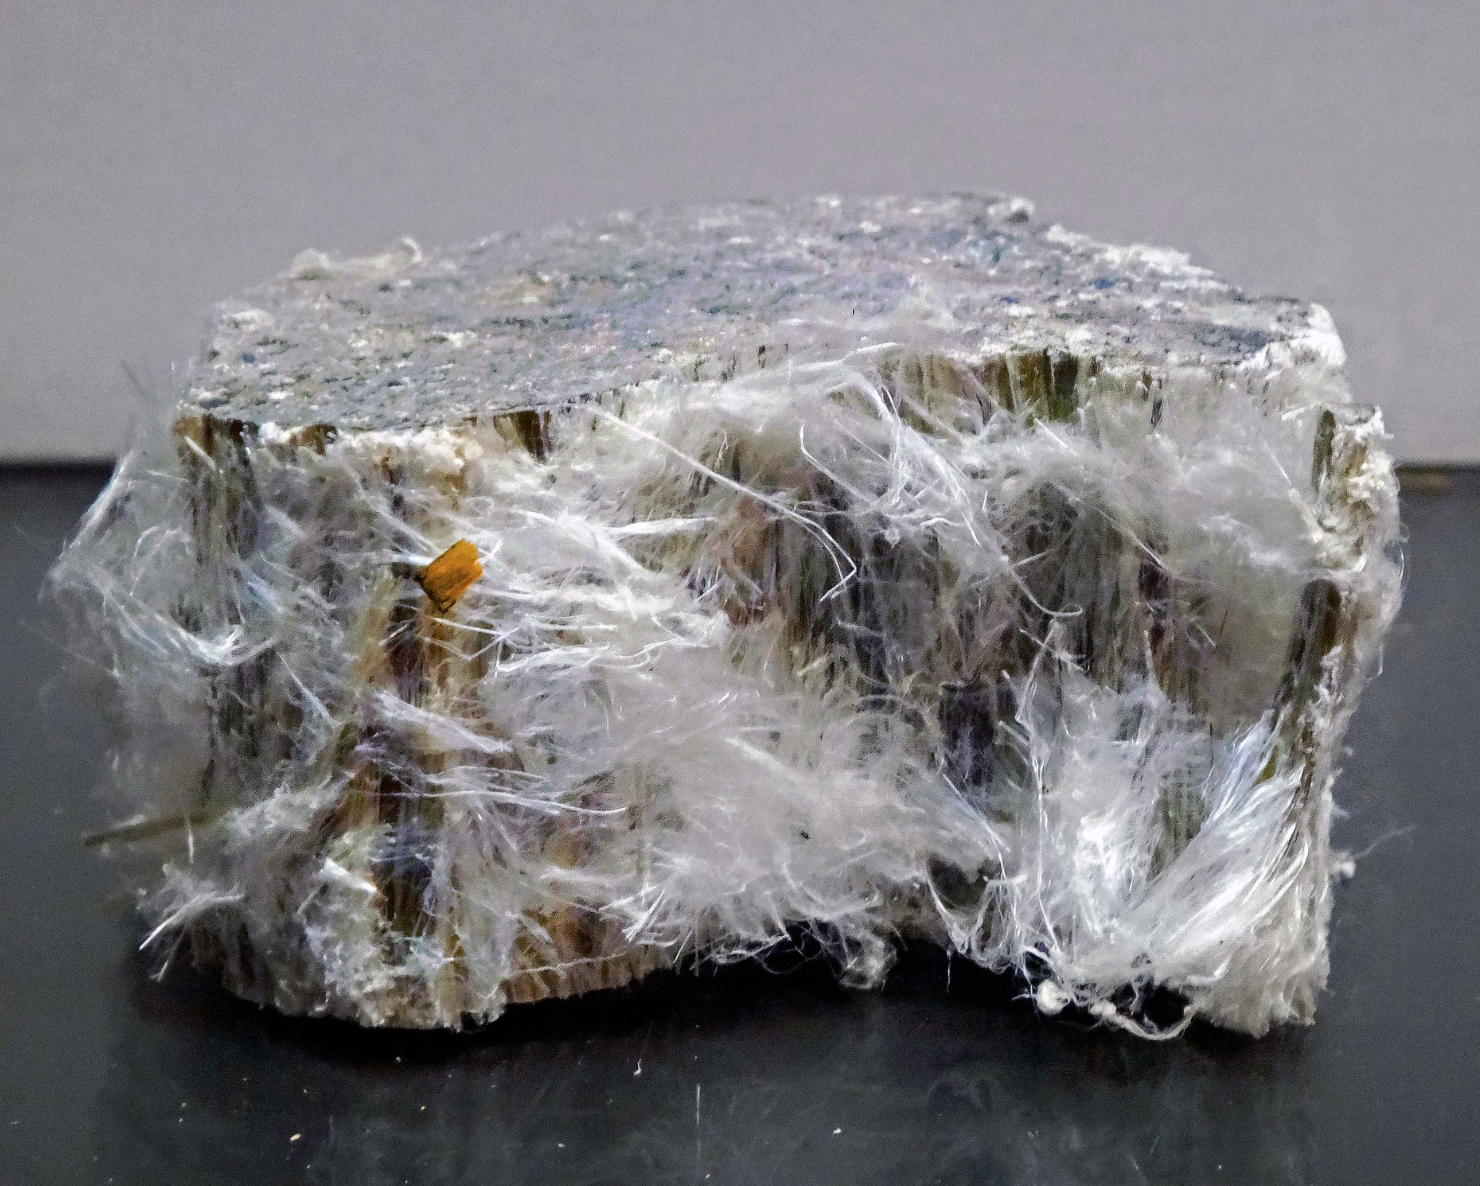
\includegraphics[width=.35\textwidth]{images/chapter1/chrysotileFullSize}
}
\subfigure{
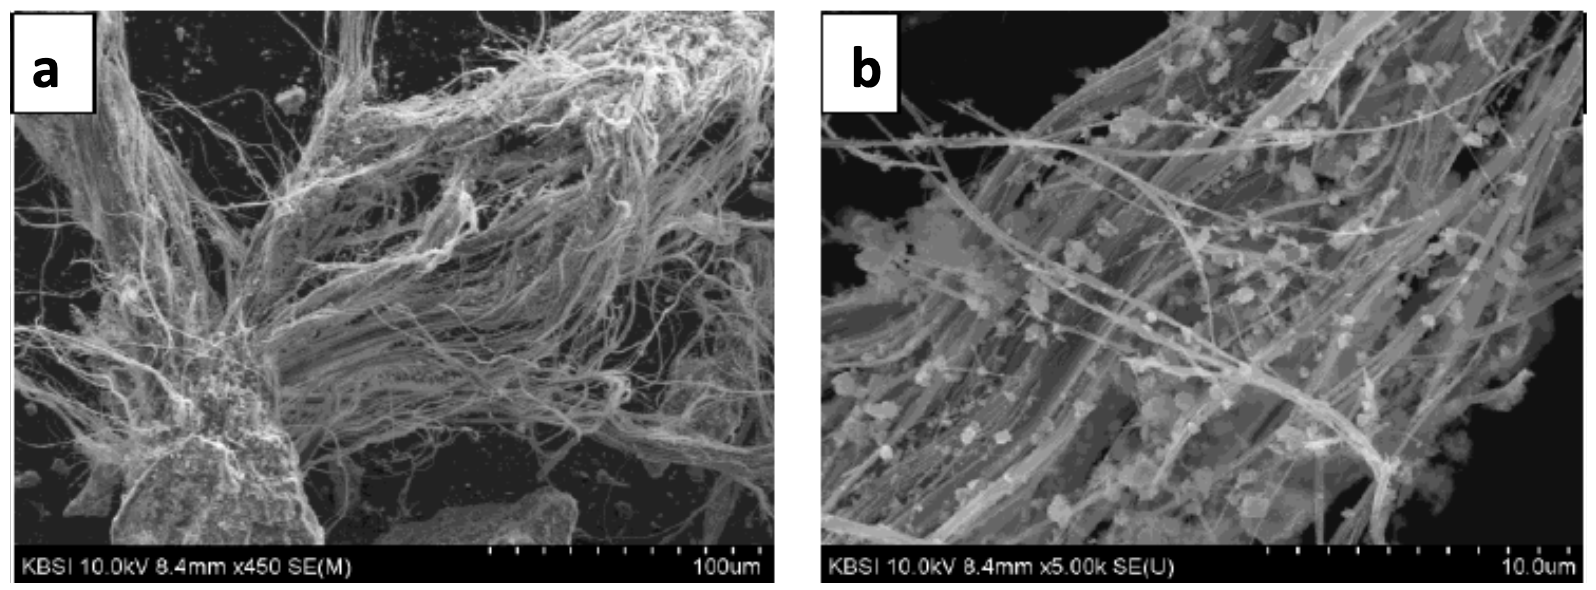
\includegraphics[width=.55\textwidth]{images/chapter1/chrysotileSEM}
}
\label{fig:chrysotile}
\end{figure}

\quad

Exposure with asbestos through inhalation or ingestion can lead to many asbestos-related diseases like mesothelioma (a type of cancer) or asbestosis (long-term inflammation and scarring of the lungs)~\cite{asbestosMaacenter, MesotheliomaWiki, asbestosisWiki}. These debilitating health effects in humans after exposure to asbestos made it very necessary to develop effective techniques and methods to detect and quantify asbestos in a variety of materials and in the environment. There is no one superior method in asbestos detection but rather a large number of different methods in preparation and analysis that need to be adapted to the specific task at hand. \\

Convolutional Neural Networks (CNNs) have become the first choice in many areas such as image recognition, classification, object detection, identifying faces and others. Although CNNs have existed already since 1988, recent progress in computational power through the immense parallelization of GPU's have made deeper and wider neural networks possible. In 2012, Alex Krizhevsky and his group won the ImageNet Large Scale Visual Recognition Challenge (ILSVRC)~\cite{krizhevsky2012imagenet, imagenet} with a CNN and since then research into this type of neural networks has increased drastically with new CNNs surpassing human-level performance in many fields. \\

A convolutional neural network is a specific type of Artifical Neural Network (ANN) which gets its name from trying to model a biological neural network. It consists of many neurons often called nodes or units that process information in a feed forward manner. A neuron receives input from other neurons (similar to brain cells that are interconnected with other brain cells) building up a huge network. This input from many different neurons is weighted and processed before forwarding the information (output) to the next neuron. A Multi Layer Perceptron (MLP) is a network consisting of fully connected layers, meaning that every neuron in one layer is connected to all the neurons in the subsequent layer. \\

For image classification, having fully connected layers of hidden units is not very useful, since no spatial information can be retrieved from the image itself. Convolutional neural networks are able to scan through the image and retrieve spatial feature maps, that find characteristic patterns throughout the image. These convolutional layers are connected to form a bigger and deeper network. These networks can be represented as directed acyclic graphs (DAGs). \\

So far, there is almost no research done on the combination of Deep Learning (DL) applied on asbestos detection from SEM images. Finding relevant publications in this field of research was very difficult at the time of writing. Although there is some work done on DL in combination with SEM images, or transfer learning applied to medical images, there is still a need to further investigate how deep learning can be used to detect asbestos fibers.\\


% It was very difficult to find publications that were relevant enough to be used for my thesis, or that came up with very original ideas to be further investigated. Although there is much research on transfer learning applied to medical images, there  is still a need to further  investigate how deep learning can be used to detect asbestos fibers.

\section{Motivation}

Asbestos detection is a very cost intensive and error prone process that needs a high degree of experience by the expert. The laboratories conducting the testing of samples need to be certified and even then, there is no guarantee that asbestos will be correctly identified. Reducing cost and error rates are important goals in order to make asbestos testing readily available, thus leading to a safer environment.\\

The motivation of this thesis is to create a model that is able to perform equally well as humans do but at a highly reduced cost; to understand how this model learns and thus increase user's trust in it; to develop strategies on how to further improve generalization and performance of the model without overfitting to the already seen data. \\

\newpage

I also want to inspire further research into the field of transfer learning on microscopic asbestos images and provide ideas and advice on how to achieve even better performance on this specific task.\\


\section{Study Subject}


The goal of this thesis is to study and evaluate the applicability of deep learning coupled with transfer learning to SEM images for asbestos detection. I will investigate different CNN architectures and network modifications, apply transfer learning from ImageNet~\cite{imagenet} on them and compare all the architectures against each other. Applying transfer learning could be challenging since the pre-trained weights are transferred from a completely different source domain. Nonetheless, it will be a central part in this thesis because only a very small dataset of asbestos images is available. I will try to visualize what the network has learned in order to further improve on the architecture through modifications and to increase user's trust in this model. Several deep learning methods like data augmentation, cropping and dataset variations will be applied in a exploratory manner to the different architectures and their impact will be evaluated. \\

First, a good baseline needs to be established by using basic CNN architectures like AlexNet~\cite{krizhevsky2012imagenet}. The inter-rater agreement rate will additionally give a measure of how difficult it is to find mutual consensus in this task. These two metrics are the minimum requirements and further improvements will be measured against them. The current state-of-the-art architectures are all based on natural images as found in the ImageNet dataset from the ILSVRC. That raises the question if the current architectures are really optimal for the asbestos detection problem. In order to achieve good accuracies, profound understanding of the different layers of a CNN and how they interact with each other is necessary, thus providing the tools needed to perform alterations on them to increase performance while reducing complexity. Several modules in DeepDIVA~\cite{deepdiva} will need modifications and re-implementations. Transfer learning will be applied in order to start with already pre-trained weights. Fine tuning will be always performed for all layers instead of only fine-tuning the last layer.\\

The research challenge is to study the applicability of deep learning models with transfer learning from ImageNet on a very small dataset of highly specialized SEM images of asbestos.\\

\section{Microscan Service SA}

This master thesis is done in collaboration with Microscan Service SA, a certified laboratory and independent scientific center for scanning electron microscopy and microanalysis located in Lausanne, Switzerland. Microscan Service SA generously provided the dataset of SEM images of asbestos fibers used in this project. They also provided a ground truth sample of about 180 characteristic asbestos structures to learn from.

\section{Outline}

The remainder of this thesis is organized as follows. Chapter 2 explains shortly the dataset used for this task, go into related work and make an analysis of which frameworks and tools are currently used. Chapter 3 will explain CNN in detail and go through all the architectures used in this thesis and explain them. Chapter 4 will provide information on how the architectures are used and modified with the goal to increase performance at lower complexity. Several deep learning techniques are introduced and explained. Chapter 5 will evaluate transfer learning in great depth, since it is one of the main contributions of this thesis. Chapter 6 will evaluate changes to the architectures, cropping methods and dataset alterations. Chapter 7 will go into the conclusion and future work. Chapter 8 holds the Appendix with more complete visualizations and the link to the GitHub repository, where all implementation is made publicly available.\\


\chapter{Analysis}

In this chapter I will shortly describe the dataset provided for this task, go over related work, then describe the frameworks and tools that are available. In the end, I draw a conclusion and decide on how to proceed.

\section{Dataset}

The provided dataset consists of about 2'000 microscopic images with and without asbestos fibers. The images come in two different dimensions and different qualities. Most of the images are 1024 by 1024 pixels and using up 1.1 MB of disk space but some are in 1024 by 768 pixels and use only around 700 kB of disk space. The smaller images were originally in TIF format which needed to be converted into PNG format for better being able to load them into python objects. All images are in grey color space. Since all architectures have been originally trained on color images, the image is transformed into an RGB tensor during dataset preparation. All gray space values ranging from 0 to 255 are simply copied into each channel of RGB. In Figure \ref{fig:asbestos_examples} three images with a asbestos fiber are shown whereas in Figure \ref{fig:non-asbestos_examples} three images without asbestos are shown.\\


\begin{figure}[h]
\centering
\caption{Three examples of images with asbestos fibers. On the left, the asbestos fibers are clearly visible, in the middle it's much harder to find them. In the right image there might be none, although the image is labeled as having asbestos in it.}
\subfigure{
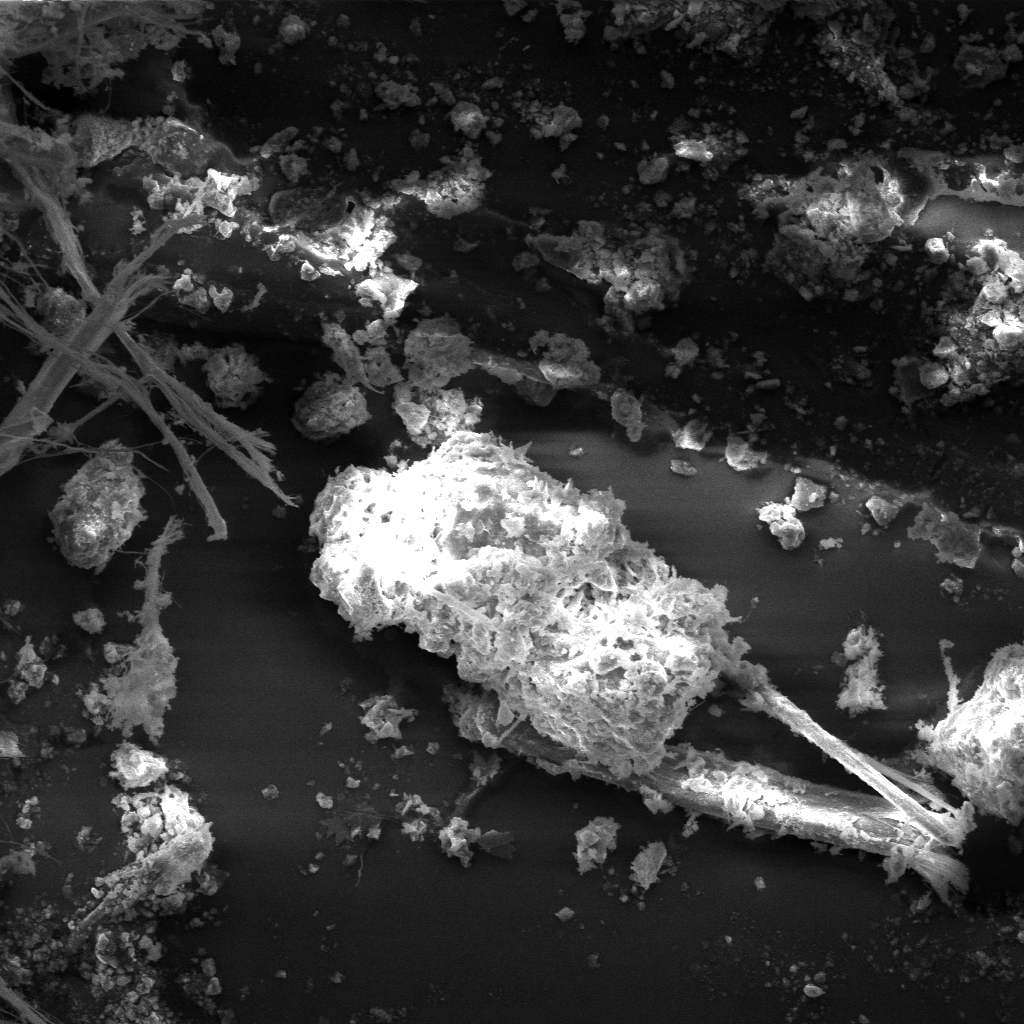
\includegraphics[width=.3\textwidth]{images/chapter2/asbestos_one.png}
}
\subfigure{
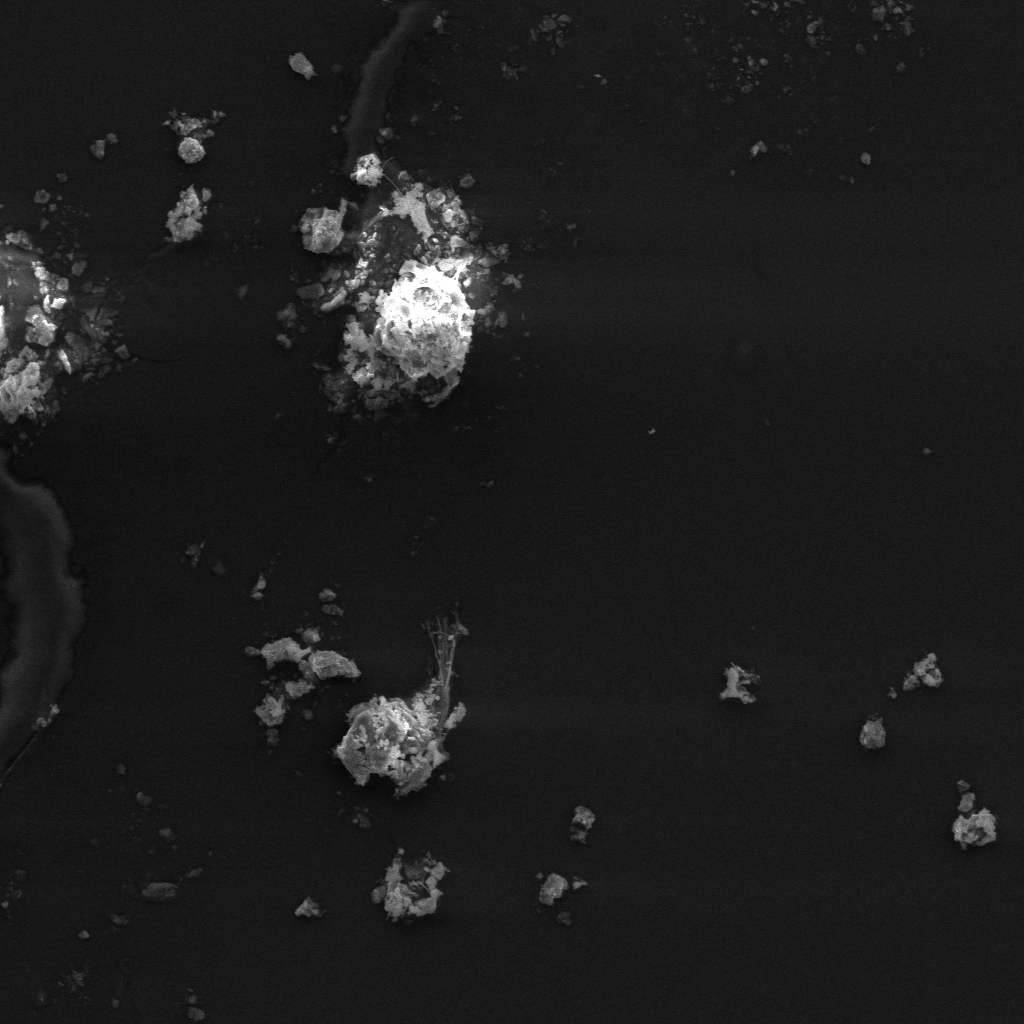
\includegraphics[width=.3\textwidth]{images/chapter2/asbestos_two.png}
}
\subfigure{
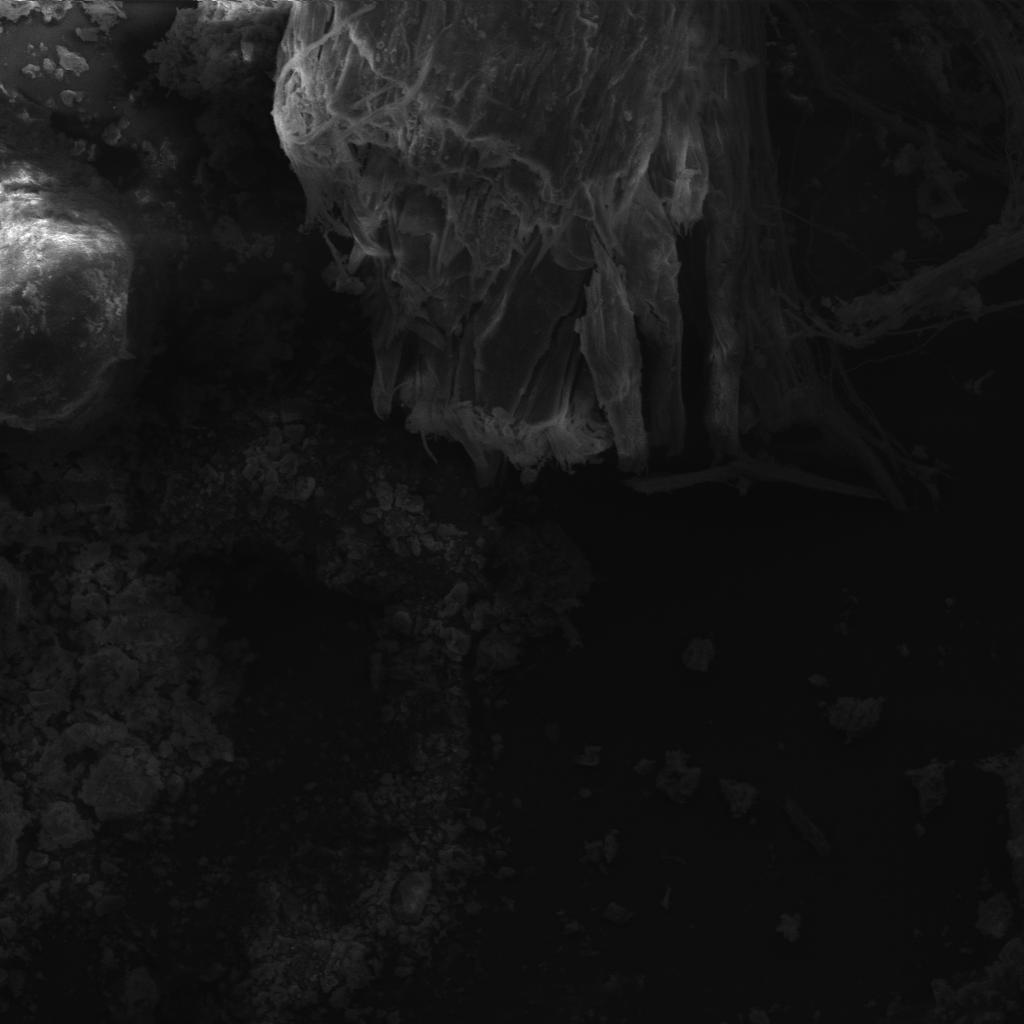
\includegraphics[width=.3\textwidth]{images/chapter2/asbestos_three.png}
} 
\label{fig:asbestos_examples}
\end{figure}

\begin{figure}[h]
\centering
\caption{Three examples of images without asbestos fibers. On the left image, there is clearly no asbestos to be found. In the middle and left image it's already much more difficult to be certain that there is none.}
\subfigure{
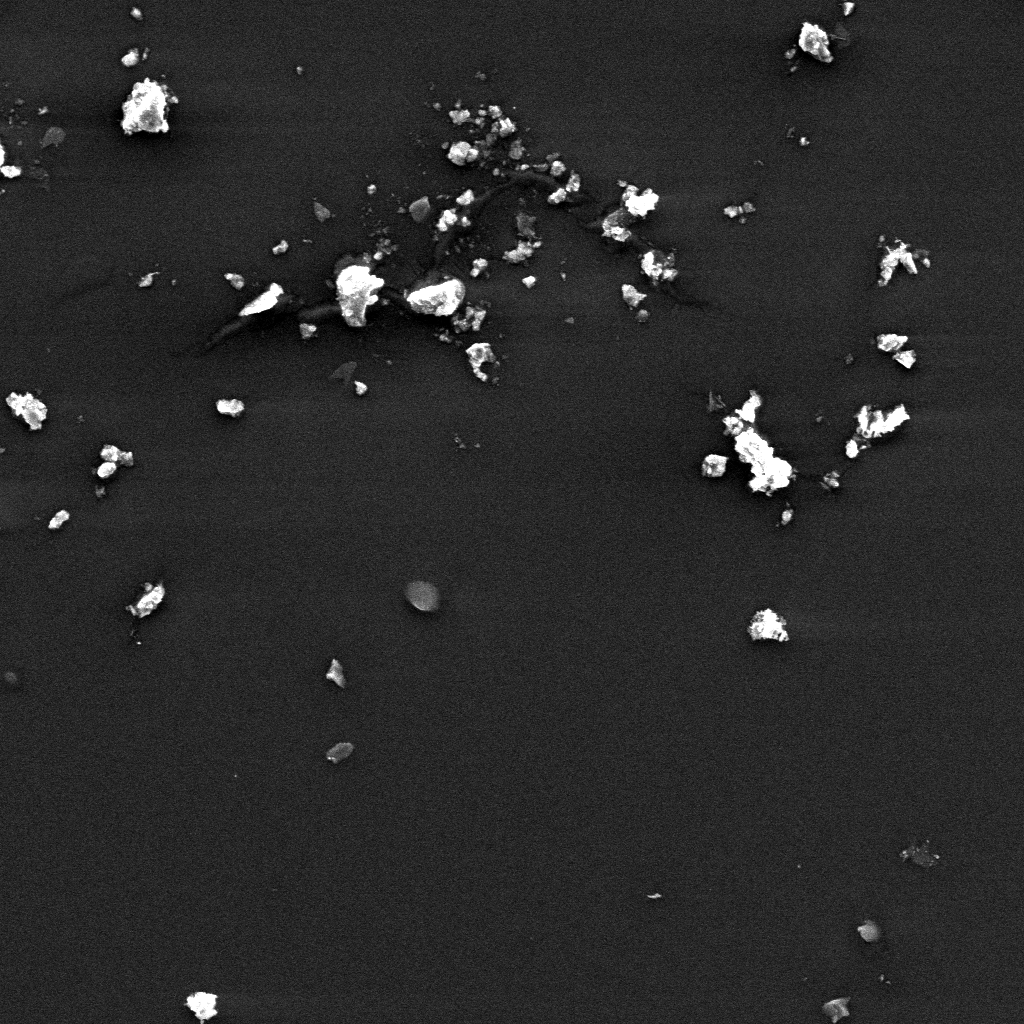
\includegraphics[width=.3\textwidth]{images/chapter2/non-asbestos_one.png}
}
\subfigure{
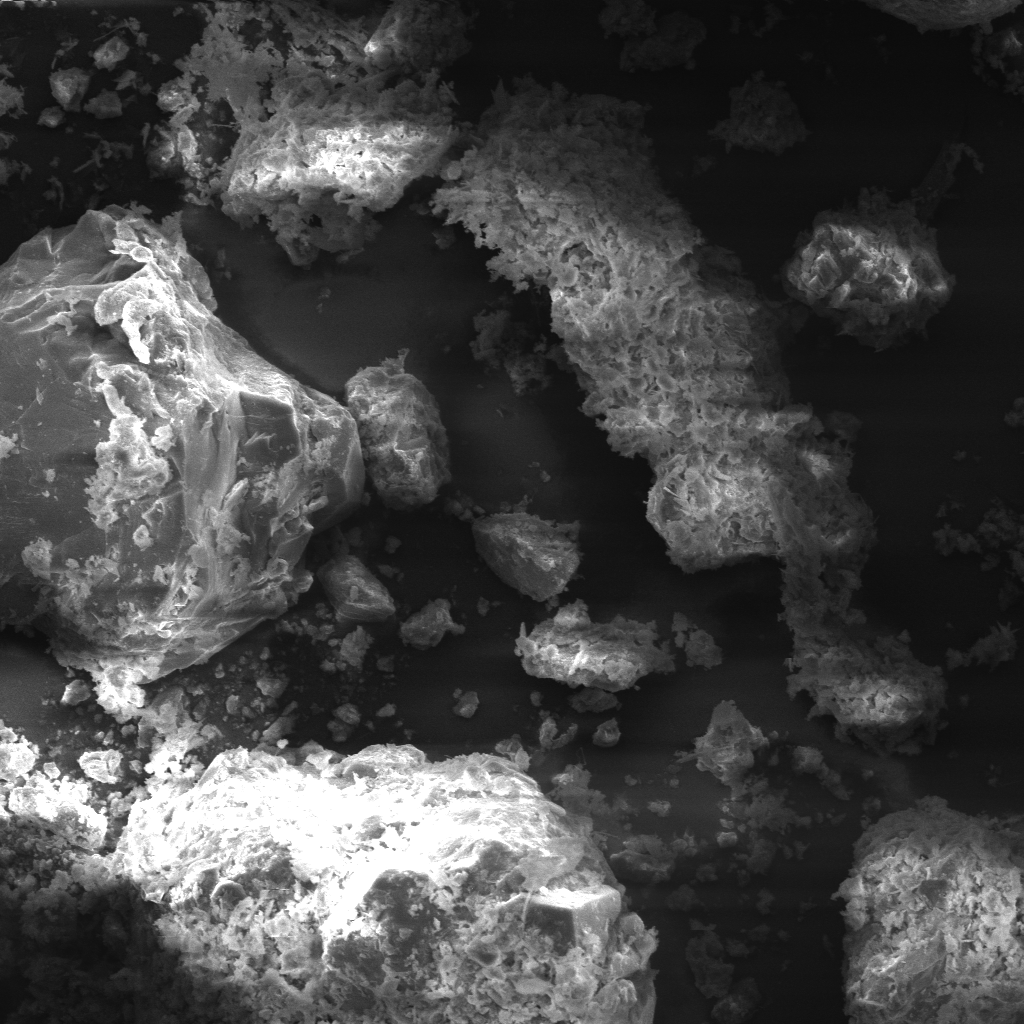
\includegraphics[width=.3\textwidth]{images/chapter2/non-asbestos_two.png}
}
\subfigure{
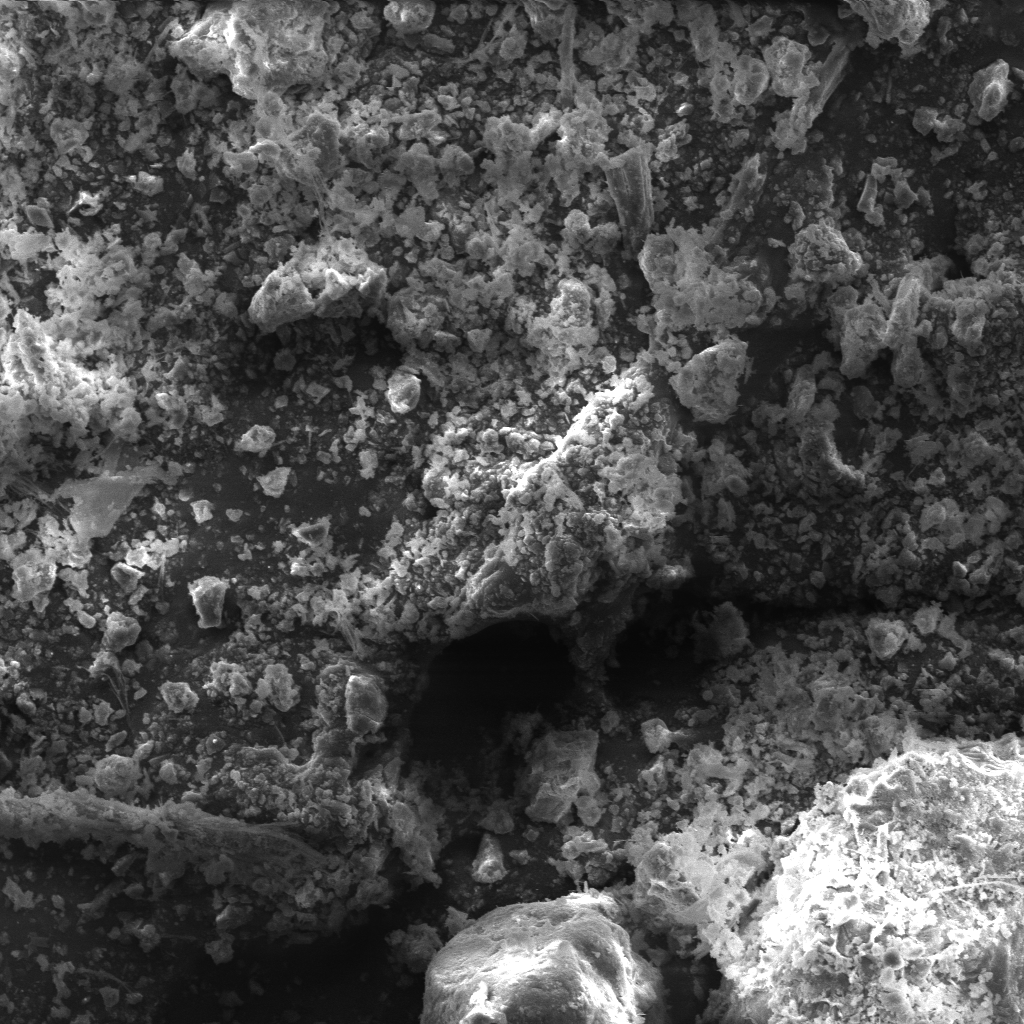
\includegraphics[width=.3\textwidth]{images/chapter2/non-asbestos_three.png}
}
\label{fig:non-asbestos_examples}
\end{figure}

With the dataset a ground truth folder was provided with 116 images pre-labeled has having asbestos fibers in them or not. From these 116 images the remaining images needed to be manually labeled. Some of the later labeled images were checked by the laboratory but Figure \ref{fig:wrong_asbestos_labeling} shows that even that leaves much space for errors.  According to the laboratory, the image shown in Figure \ref{fig:wrong_asbestos_labeling} has no asbestos in it. Nonetheless, there are several areas where asbestos-like structures emerge once the image is made brighter with a photo-editing tool, especially a long fiber on the left side of the image marked by two arrows. Brightening, sharpening and other simple editing tools are often used prior to classification to make the structures more visible. This is to show, that the labeling will most certainly have errors in it and that some images might look like having asbestos fibers in it but actually don't and the other way around. In order to be sure, the probes are examined with additional methods in a second phase that is not part of the master thesis. Therefore one of the main goals of this thesis is to be able to label all uncertain images for further examination. That means that the rate of false negatives should be as low as possible.

\begin{figure}[h]
\centering
\subfigure{
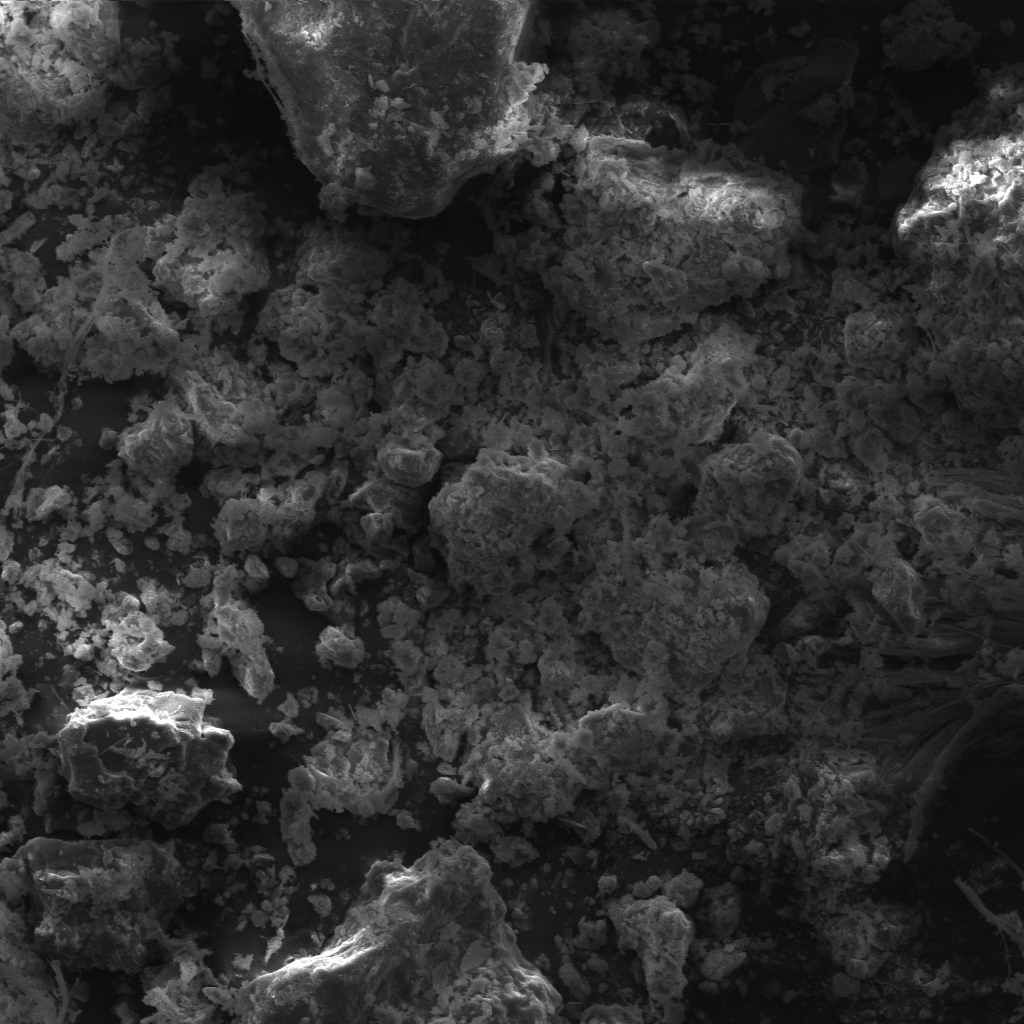
\includegraphics[width=.4\textwidth]{images/chapter2/probably_wrong_label.png}
}
\subfigure{
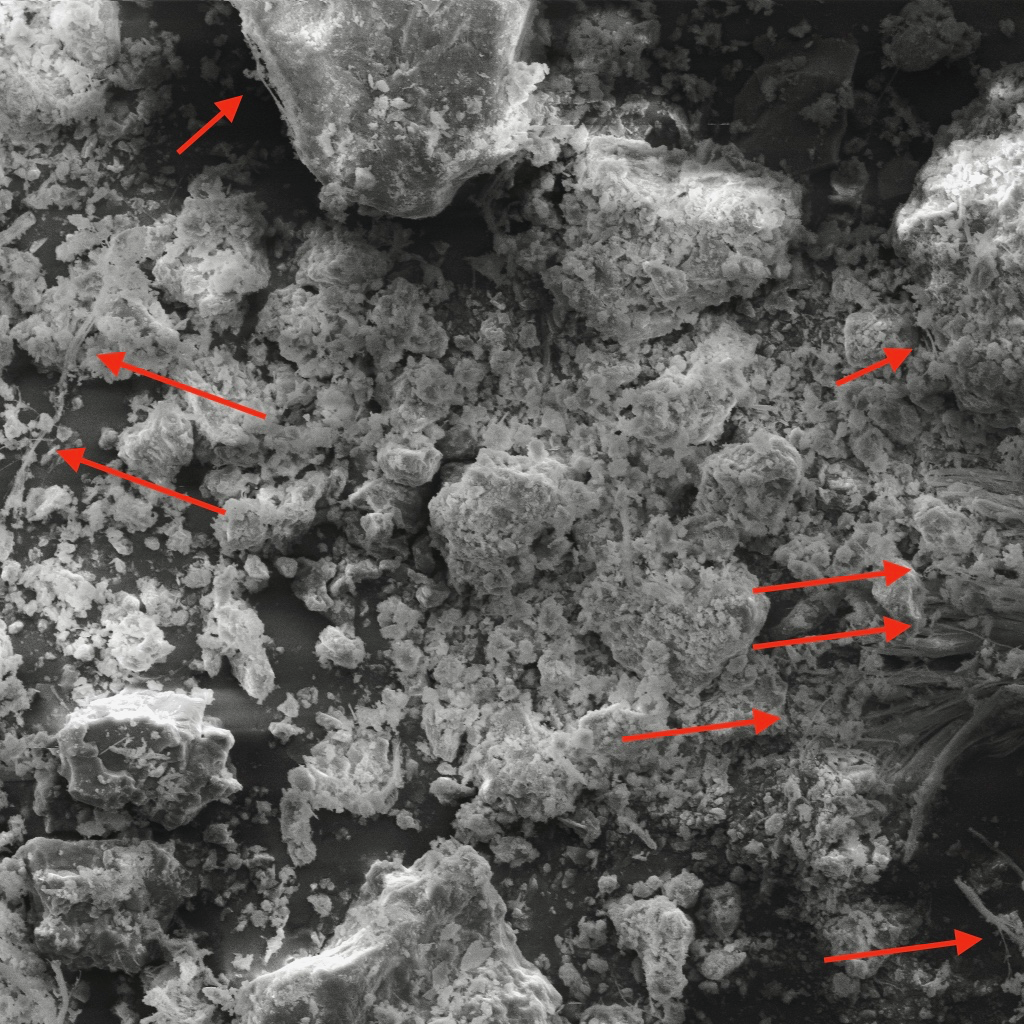
\includegraphics[width=.4\textwidth]{images/chapter2/probably_wrong_label_edited.png}
}
\caption{After brightening up the image and looking at it carefully, many different asbestos like structures emerge.}
\label{fig:wrong_asbestos_labeling}
\end{figure}

\section{Related Work}

There are many different forms of asbestos that occur in different materials and environments, therefore the detection and quantification methods are quite different as well, although most of them are based on microscopic images. After the samples have been collected, trained experts need to quantify and classify the fibers in order to assess the contamination and risk factors to humans. The reason for that is that not all asbestos fibers are equally toxic to humans. The structure needs to be manually checked and matched exactly to a set of predefined and standardized characteristics, also called templates. This process is very time intensive and costly and therefore automated detection and counting methods are being developed. The most important and widely used methods for detecting asbestos from air samples are e.g. phase contrast microscopy (PCM), transmission electron microscopy (TEM), scanning electron microscopy (SEM) as seen in Figure \ref{fig:chrysotile}, and polarized light microscopy (PLM) \cite{perry2004discussion}. These techniques are mostly adapted for soil samples although soil samples pose many new problems like standardized preparation of the samples. Air samples are much cleaner and the asbestos fibers can be counted more easily without noise interfering, thus the results are more accurate and counts are rather reproducible. With soil samples, there is much more debris in the samples and getting a homogenous sample out of a bigger object that can generalize to the whole is one of the biggest problems. Figure \ref{fig:sampleprep} shows how a very simple sample preparation could look like. \\

\begin{figure}[h]
\centering

\subfigure{
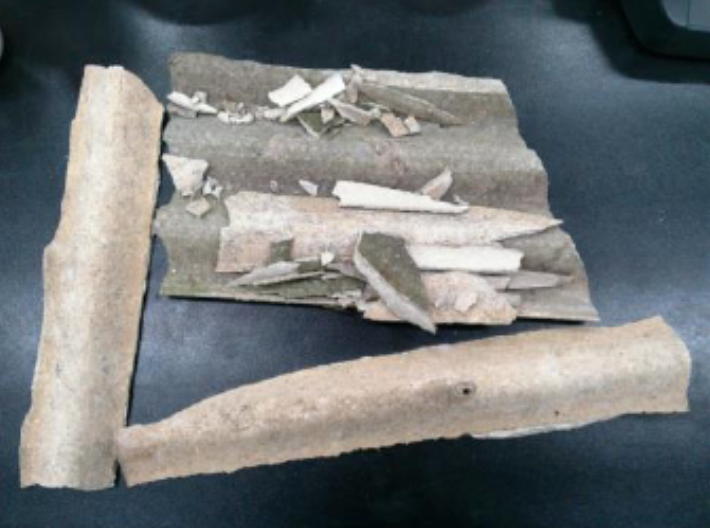
\includegraphics[width=.4\textwidth]{images/chapter2/SamplePrepOne}
}
\subfigure{
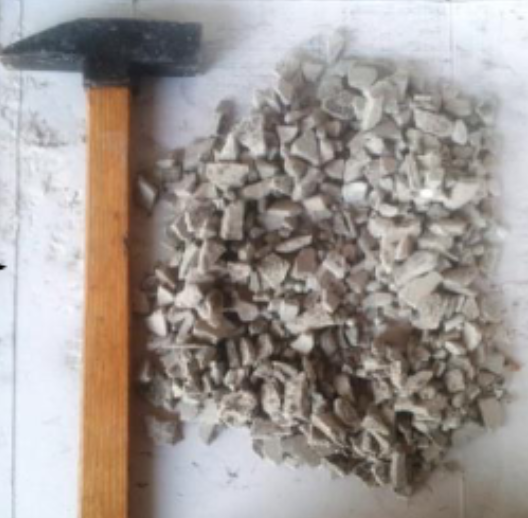
\includegraphics[width=.35\textwidth]{images/chapter2/SamplePrepTwo}
}
\subfigure{
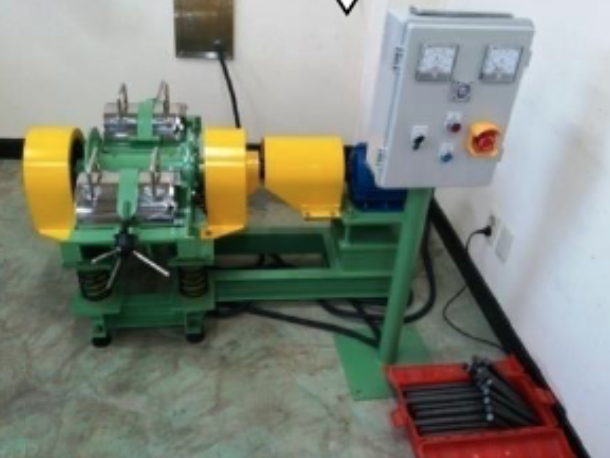
\includegraphics[width=.4\textwidth]{images/chapter2/SamplePrepThree}
}
\subfigure{
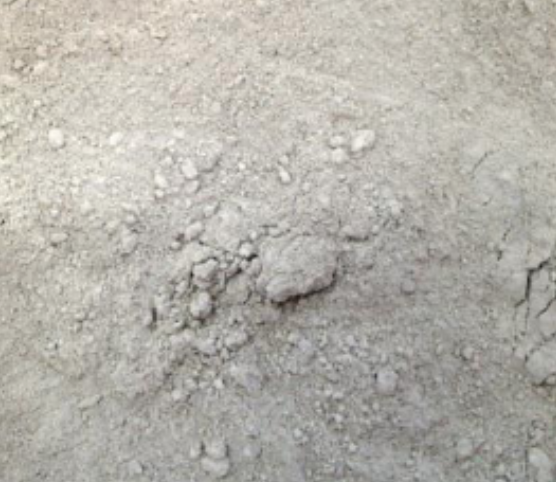
\includegraphics[width=.35\textwidth]{images/chapter2/SamplePrepFour}
}
\caption{On the upper left image the raw material is seen that needs to be screened for asbestos. In the upper right image it has been processed in a first step manually. In the left lower image a crusher is seen, that takes the pieces and processes them into fine grained powder seen in the lower right image \cite{mohammed2015}. }
\label{fig:sampleprep}
\end{figure}


There are many other asbestos detection methods and counting strategies like using certain proteins from Escherichia coli that binds strongly to chrysotile, which in turn makes chrysotile easily detectable with fluorescent microscopy \cite{kuroda2008detection}. Other current methods are Polarized light microscopy (PLM), X-ray diffraction (XRD) and Fourier Transform Infrared Spectroscopy (FTIR) \cite{campopiano2018inter}. In a current and rather big inter-laboratory study, 475 laboratories in Italy were tested if they could reliably detect asbestos fibers in several bulk materials using the above mentioned three methods of PLM, XRD and FTIR. Many laboratories (ranging from 3\% to 40\% depending on the material and asbestos fiber) were classified as unsatisfactory having made to many errors in the classification. The authors concluded that asbestos detection is a complex process that uses several different approaches depending on the material and that the experience and skill of the analyst is very important. Without proper training and a scientific approach, it is very difficult to classify asbestos accurately \cite{campopiano2018inter}. \\

There are still many other detections methodologies but they all rely on manual screening which is very time-intensive labor. Searching on Google Scholar leads to very few papers, that applied some sort of machine learning algorithms in combination with one of the mentioned microscopy.

Cossio et al. describe an unattended scanning electron microscopy analysis with energy dispersive spectrometry (SEM-EDS) for asbestos quantification (counting of the fibers) \cite{cossio2018innovative}. Their goal was to find an automated process to increase productivity and sensitivity. After having prepared the samples and the SEM images were taken, they needed to be binarized in order to discriminate the shapes clearly from the background. They applied thresholding for that reason and transferred the image from grayscale to a black and white image only as seen in Figure \ref{fig:binarization}.

\begin{figure}[h]
\centering
\caption{Performed binarization on the grayscale image in order to discriminate the asbestos-like structures from the background noise \cite{cossio2018innovative}. }
\subfigure{
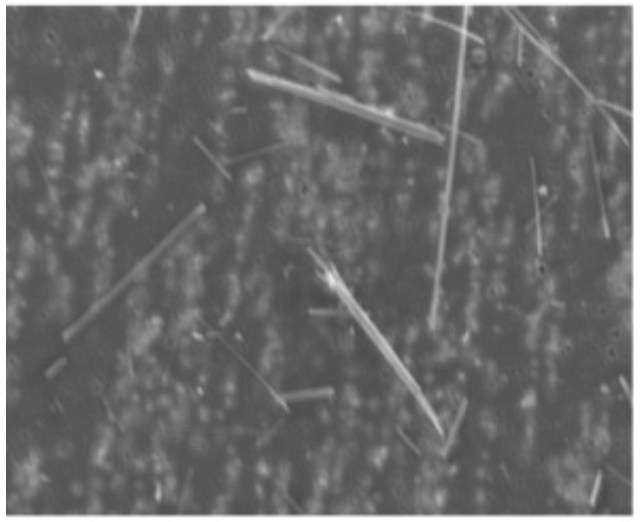
\includegraphics[width=.4\textwidth]{images/chapter2/image_original}
}
\subfigure{
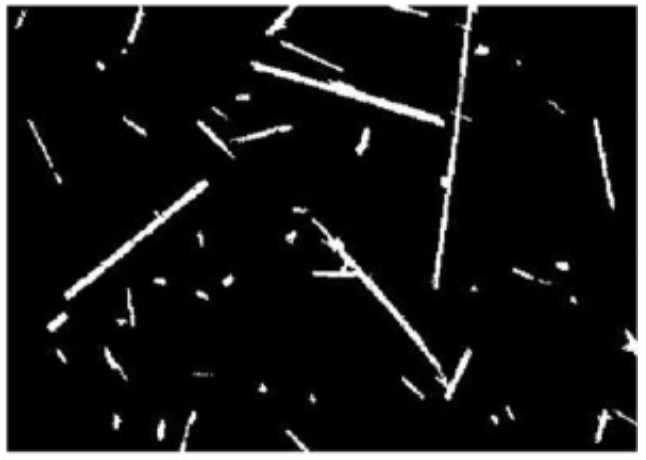
\includegraphics[width=.4\textwidth]{images/chapter2/image_binarized}
}
\label{fig:binarization}
\end{figure}

Then EDS is applied on the areas found from step 1 in order to save analytical time. Fiber morphology is then used to analytically discriminate between asbestos fibers and other minerals looking similar to asbestos. That includes length, width and aspect ratio (length/width) of the mineral structure. For Chrysotile Cossio et al. achieve 49.88\% accuracy in counting the fibers with feret diameters and 78.66\% with equivalent rectangle (ER). Both are morphology methodologies \cite{cossio2018innovative}.

Kawabata et al. use X-ray diffraction to obtain the image and dispersion staining methods to evaluate the asbestos-like structures \cite{kawabata2009asbestos}. The dispersion staining method is a visual inspection in which white light passing through the asbestos structure is dispersed into several colors. For chrysotile structures, the dispersion colors are in the range of red-purple to blue. Filed interviews revealed that using this method of X-ray diffraction and dispersion staining no more than 10 samples can be examined daily. The goal of Kawabata et al. was to automate this process by examining color changes of two same images in response to dispersion staining and polarization. Relative to the aspect ratio of the fiber they achieved detection failures of chrysotile asbestos ranging from 0.35 to 0.65. The average number of incorrectly identified asbestos fiber was approximately 1.2 for chrysotile \cite{kawabata2009asbestos}. 

Moriguchi et al. used a similar approach as Kawabate et al. and used the color information from polarization (dispersion) coupled with Support Vector Machine (SVM) as the computer-based detector \cite{moriguchi2008asbestos}. To get the different properties the sample needs to be captured from two different angles. Since the two images need to be matched, the difference in angle needs to be computationally corrected for. They also found that applying SVM on every single pixel leads to many false positives and false negatives. Therefore they propose to use Conditional Random Field (CRF) on SVM outputs in order to also take the neighboring pixels into account. Miriguchi et al. reach an accuracy of 71\% with the SVM method and 78.9\% with the SVM method coupled with CRF.

Robson et al. developed a method to detect and count asbestos fibers from air samples \cite{robson2018fiac}. In contrast to soil samples, air samples are much cleaner and have less noise making the detection and counting process more easy and objective. Robson et al. used Mak R-CNN described in \cite{he2017mask} that adds a mask prediction onto the image itself showing regions that likely include the object of interest. Since Robson et al. had not enough data on hand, data augmentation and transfer learning were also applied. They were able to accurately detect 70\% of the fibers in a test set of 50 images  \cite{robson2018fiac}. \\


All in all, it is very difficult to compare the results with each other since every group uses different samples with different pre-processing methods on the image and detection or counting algorithms. It should be noted that none of the mentioned works reached an accuracy of 80\% or higher.


\section{Deeplearning Frameworks}

There are two main Deep learning Frameworks that can readily be used. Tensorflow \cite{tensorflow} which was originally developed by researchers and engineers at Google Brain and is based on Theano and PyTorch \cite{pytorch} that was built by researchers at Facebook. They are both open source and free to use, but the flavor is quite different. While TensorFlow uses static computational graphs that need to be built prior to compilation and run in their run engine, PyTorch uses dynamic computational graphs that can be more interpreted than compiled. Programming in PyTorch is much more pythonic whereas in TensorFlow the user needs first to get used to the Tensorflow way of doing things. Like building the whole computational graph in advance, using placeholders for all weights and variables, then creating a session in which the graph can be executed. Debugging in Tensorflow is more difficult since it needs at least two different debuggers to be used. One for the tensors and their values, and one for the python code itself. That makes it much less intuitive to simply debug the underlying code while keeping track of all tensors. In PyTorch, the native debugger may be used for the whole codebase, including all the variables and weights. Data parallelism is much easier to use in PyTorch since the distribution of the code and data onto all the GPU's happens automatically. Whereas in Tensorflow much more manual work and careful thought need to be applied to achieve the same behavior. Since PyTorch is one big framework it gives more the feeling of working with one framework that uses a very pythonic way to handle things. TensorFlow, on the other hand, is more like an aggregation of many libraries that work together to achieve a common goal. Although that was the case in early 2018 things are changing very fast for these frameworks. Tensorflow was much better for production environments but with PyTorch version 1.0 this advantage is closing fast \cite{pytorchOnePointZero}. Table \ref{tbl:DeepLearningFrameworks} summarizes the different qualities of both frameworks at the start of the Master thesis in late summer 2018. \\

\begin{table}[t] \centering
\ra{1.3}
\caption{Different qualities of the Deeplearning frameworks: PyTorch and Tensorflow)}
\begin{tabular}{@{}rrr@{}}
\toprule & PyTorch & TensorFlow \\
\midrule
Open-source									& + & + \\
Dynamic Computational Graph			& + & -  \\
Static Computational Graph				& - & +  \\
Easy Learning Curve							& + & -  \\
Fast developing of new Models			& + & -  \\
Production Environment					& - & + \\
Developer Community						& + & + \\
Native Visualization							& - & +  \\
Debugging										& + & -  \\
Data-Parallelisme								& + & -  \\
Framework-Feeling							& + & -  \\
Library-Aggregation							& - & +  \\

\bottomrule
\end{tabular}
\label{tbl:DeepLearningFrameworks}
\end{table}

There are some higher level frameworks like Keras \cite{keras} and DeepDIVA \cite{deepdiva} that enable many more things and faster development. Keras is built on top of TensorFlow and has many models pre-implemented. It enables the developer to very quickly start modeling a problem or apply already present architectures to new data. It does not allow the same flexibility as TensorFlow but if a new architecture needs to be designed from scratch it is done in TensorFlow than made available on Keras as to use on different datasets or different tasks. A possible counterpart for Keras is DeepDIVA that was built on top of PyTorch and also provides pre-implemented architectures or allows to include them in a straight-forward manner. It tackles some of the disadvantages of PyTorch versus Tensorflow like including TensorBoard Visualization to PyTorch. Development in DeepDIVA is also very pythonic and does not actually change at all since it is very tightly integrated into the PyTorch framework. Creating new architectures is or altering existing ones is straight forward.

\section{Tools}

Apart from PyTorch and DeepDIVA there is need for some other tools as well. Results and data need to be visualized and some optimization tools might be better than others.

\subsection{Visualization}

WIth CNN's it is very difficult to really know what they have learned. There are several examples that an architecture performed exceptionally well on the test set but later it was found out that it didn't really recognize the object itself but some other characteristics unrelated to the studied class. This is especially important when working with only a few classes. It is indeed very unsatisfactory from a scientific standpoint to use the accuracy alone to determine if an architecture is well suited for a problem or not. Even with other statistical values added, it still lacks a deeper understanding. There are several methods on how to study what a model really learns and to visualize it. Since visualizing what the network learns is still quite a young filed of research, its quite difficult to find good libraries that can be applied to the problem. I will implement the visual toolbox by Utku Ozbulak \cite{viztoolbox} into DeepDIVA and draw conclusions from these visualizations. It remains unclear if applying this library to other architectures than AlexNet and VGG will work. From the insights gained, modifications to existing architectures might be considered. 

\subsection{SigOpt}

With all deep learning approaches it is vital to fine tune the hyperparameters like learning rate, momentum and weight-decay to the architecture and problem at hand. Often considerable amount of time is invested into this process in order to reach the best possible accuracies and reach current state-of-the-art performance. Using gridsearch for optimizing the hyper parameters would require hundreds of separate runs to find good values while only checking the value range in a very sparse manner. For the first and second baseline I did actually apply gridsearch for comparison reasons. But moving forward I applied for a academic account with SigOpt \cite{sigopt} which is a company that specializes on hyper parameter optimization. They use employ Bayesian optimization which efficiently trades off exploration and exploitation of the pre-defined hyper parameters and their respective parameter space. Thus it moves quickly towards an optimal configuration that best optimizes the user defined evaluation criterion. Common practice is to use 10 to 20 runs for each parameter which needs optimization \cite{sigoptObservationBudget}. Bayesian optimization applies mainly methods from regression models and acquisition functions, that are used together to allow fast and guided configuration search \cite{sigoptBayesian}.

\subsection{PyCharm and GIT}

PyCharm \cite{PyCharm} is an Integrated Development Environment for the Python programming language and has many useful features on board like code completion, static code analysis and an own debug environment. Being able to connect through SSH with a remote server allows for modifying the remote code locally within PyCharm IDE and pushing all changes to the remote server on every save command. Remote debugging is also available with the professional license, which is free for students. Writing local scripts and integrating them with the existing PyTorch and DeepDIVA framework is easy and git is implemented directly into PyCharm which makes it easy to do almost everything within the IDE itself.
For version control, forking the original repository and adding modifications to it, GitHub \cite{GitHub} is used in combination with PyCharm and SourceTree \cite{SourceTree} as a visual GUI.

\section{Hardware}

The hardware used is provided by the Information and Communication Department Fribourg (EIA-FR) and consists of 4 Tesla K80 Graphics Cards with each 12GB of Memory and CUDA version 10.0. It is used on an Ubuntu 18.04 machine with 32 Intel(R) Xeon(R) CPU E5-2620 cores and 126 GB of RAM. 

\section{Conclusion}

For me the most important thing was the ability to work in a very pythonic way and be able to start developing my models quickly without having to learn new frameworks. Debugging is one of the most crucial things when learning how to code new problems and because of these two main reasons my choice fell towards PyTorch. Additionally, I decided to go with DeepDIVA on top of PyTorch. It gives me many of the advantages that applied previously only to tensorflow like simple visualization of the results and learning process through tensorboard, but it also gives me some very useful pre-implemented architectures to start from. \\

For the visualization of the different layers of the network I decided to go with Utku Ozbulak's visualization toolbox \cite{viztoolbox}. It is implemented in PyTorch and can be applied with some tweakings to the AlexNet and VGG models. It has many different visualization modes to chose from and is quite extensive. It also provides a heat maps for possible localization of the object. \\

Gridsearch and Sigopt were both used for hyper parameter optimization.
\chapter{CNN}

Give a short intro into CNN

\section{Design overview}

What is the architecture of CNNs`?


\chapter{Design and Implementation}


There are several goals and contributions I want to achieve. One main goal is to be able to recognize asbestos fibers in microscopic images, and show that transfer learning can be done even in this cross-domain specific task. Transfer learning is especially important, since there are only several hundred images to learn from. To achieve this, different CNN architectures are evaluated, with and without transfer learning. Also, in order to achieve better accuracy on the asbestos recognition task, I will alter the current architectures to better meet this specific task's characteristics. Data augmentation with several cropping methods and different combinations of the data set will be iterated over. As already mentioned in the introduction there is no baseline from the laboratory or any research that can be used for comparison. Therefore a new baseline needs to be established with a simple CNN. Also an inter-annotator agreement rate has been computed. In this chapter I explain and discuss the different methods used in this thesis, talk about modifications done on the architectures and dataset.

\section{Problem Description}

The provided dataset consists of about 2'000 microscopic images with and without asbestos fibers. The images come in two different dimensions and different qualities. Most of the images are 1024x768 pixels but some are in 1024x1024 pixels. Only a small subset was pre-labled and the remaining images needed to be labeled by hand, an error-prone task since I was never professionally instructed on how to do it. After labeling the images, some of them were sent back to the laboratory for checking the labeling, but there were many images, that the experts were uncertain on how to label and put them into a new folder which they called  "uncertain". From 441 images I labeled and sent the laboratory for checking 78 images came back as being suspected to contain asbestos but they were not quite sure. That's about 5.65\%. The detection of traces of asbestos by images is indeed very difficult and the error rate increases significantly as stated by the laboratory. In a next step these uncertain samples would be chemically examined to know for sure, which is beyond the scope of this thesis. In Figure \ref{fig:basic_examples} three example images are shown. One with asbestos, one without and one image with an error, that makes it difficult to be used for the training. The first dataset used includes all the images, but in later dataset alterations, these images with errors in them are removed.

\begin{figure}[t]
\centering
\subfigure{
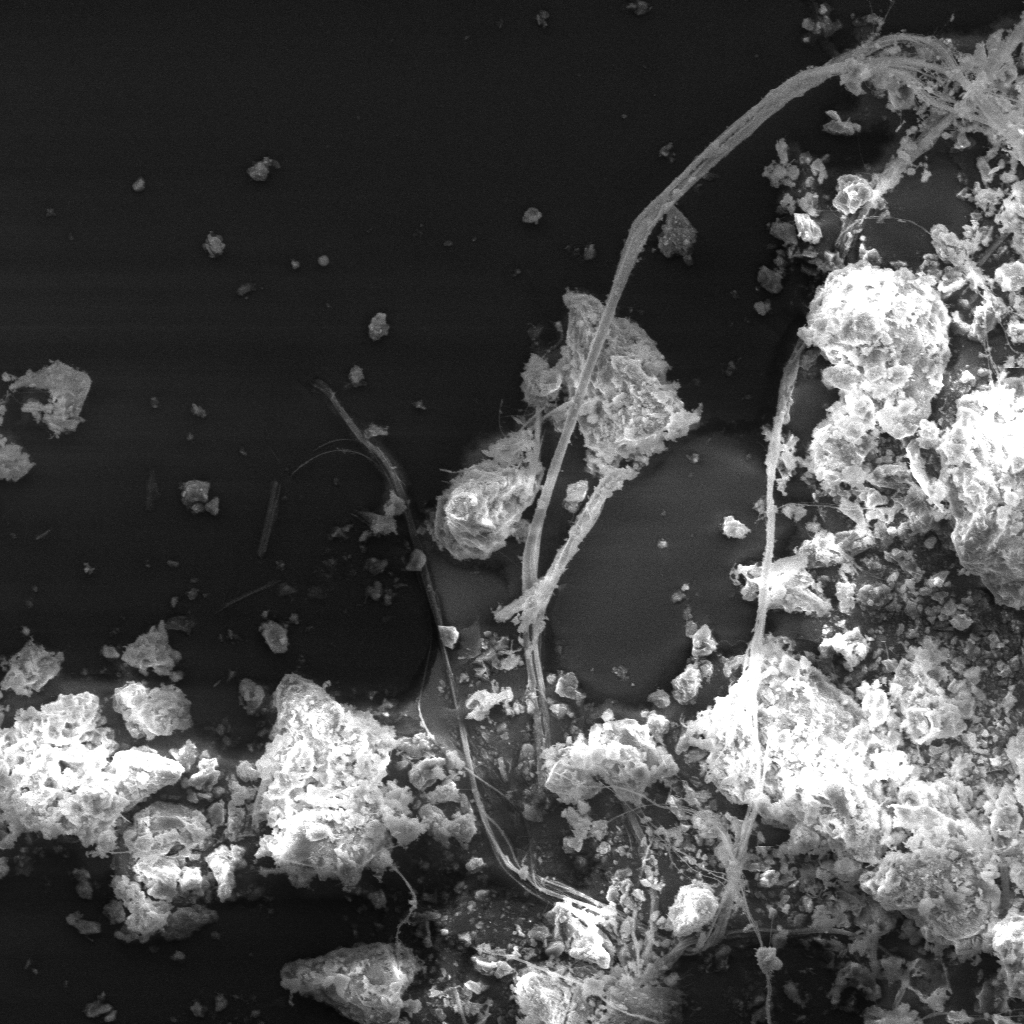
\includegraphics[width=.3\textwidth]{images/chapter4/asbestos.png}
}
\subfigure{
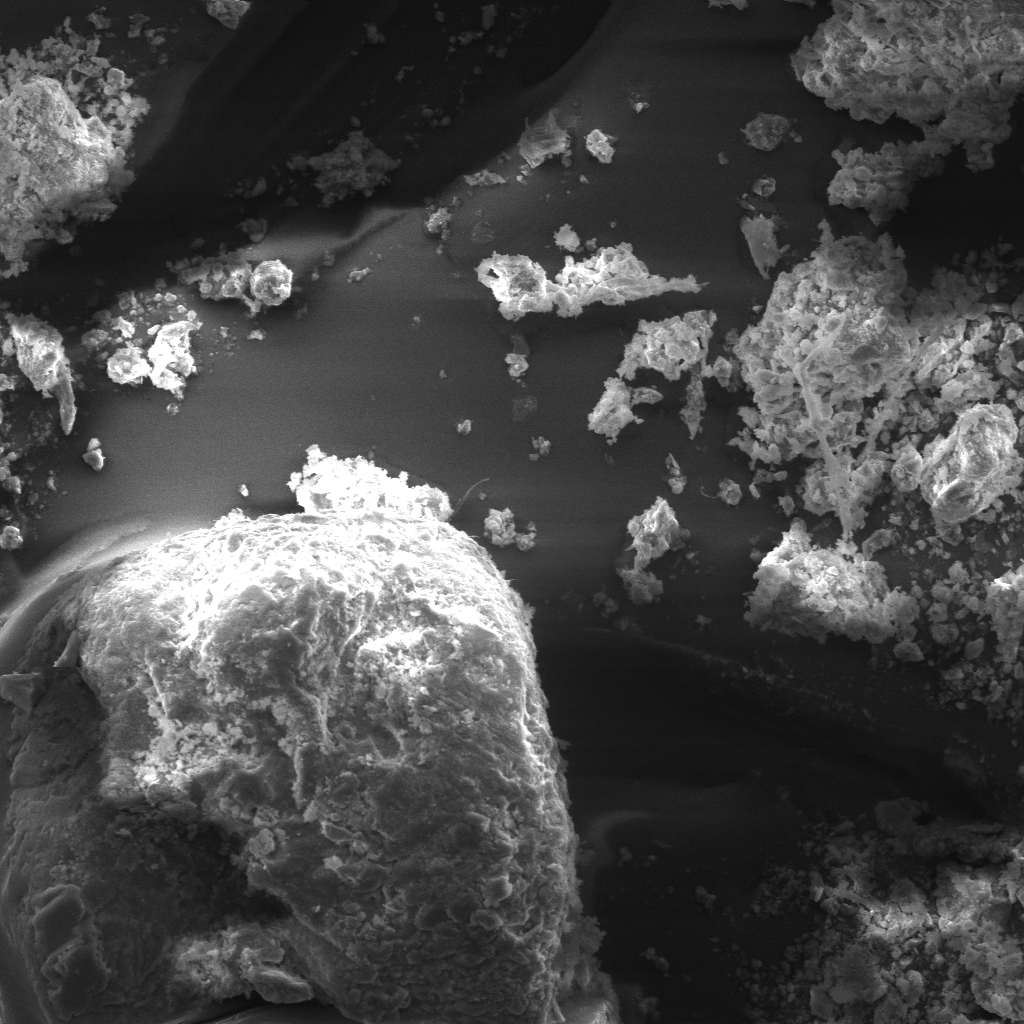
\includegraphics[width=.3\textwidth]{images/chapter4/non-asbestos.png}
}
\subfigure{
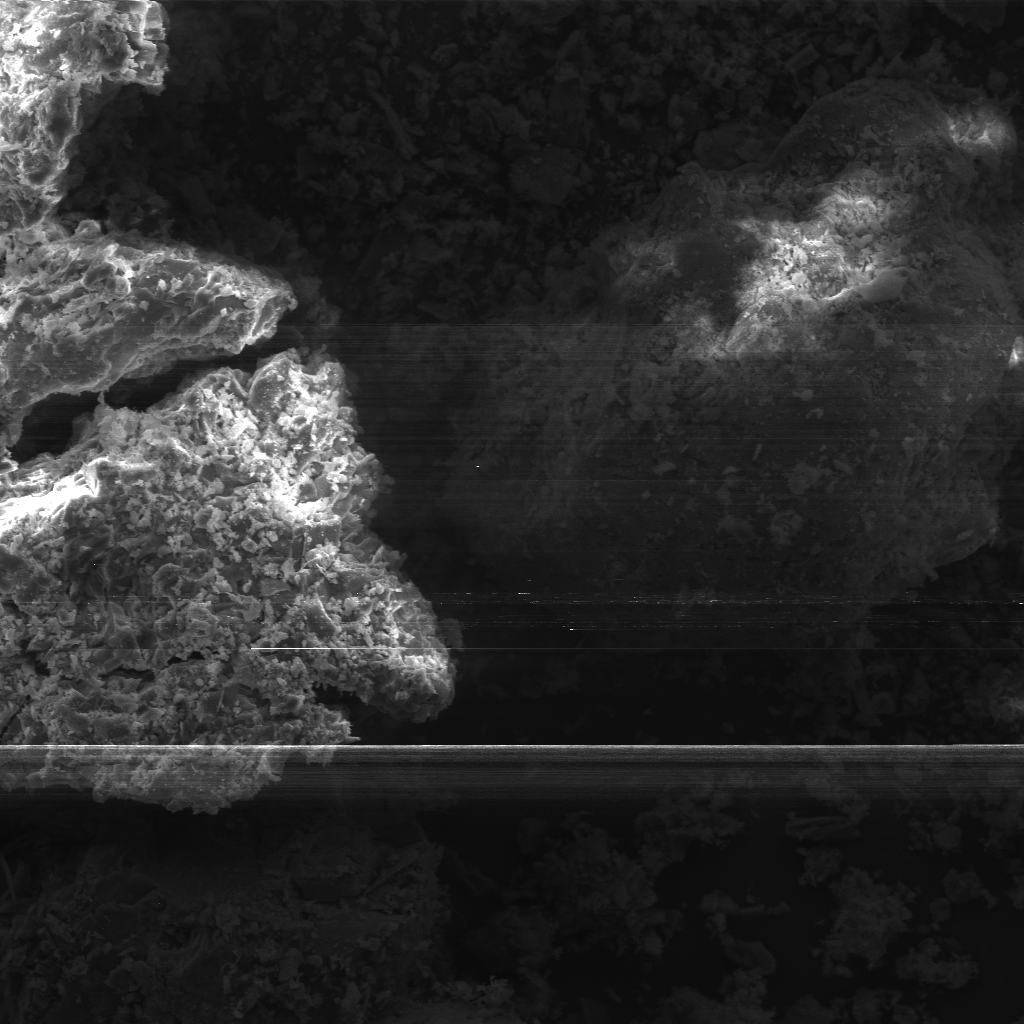
\includegraphics[width=.3\textwidth]{images/chapter4/fail.png}
}
\caption{On the left side the image shows a clear asbestos fiber, in the middle an image without asbestos is shown. On the right side, en example is provided of images that were processed with errors.}
\label{fig:basic_examples}
\end{figure}

Since the images are quite large, they will drastically increase in size, once decoded into a PIL object, or Tensor object. On the provided hardware, the memory of four Tesla K80 won't be enough to process whole images during training. Most architectures resize the images to much smaller dimensions ranging from 224x224 for ResNet to 299x299 pixels for Inception v3.

\section{Baseline}

There are two different methods used to acquire a baseline that can show improvements from changes in architectures and provide a better understanding of the data. The first one is to use a very basic CNN with grid search to find the best hyper parameters. This will give a first and low estimation of the accuracy that can be achieved. Also it provides a minimum requirement of this thesis, to improve on that performance. The other method is the inter-agreement rate or Randolphs' kappa which is a chance-adjusted measure of agreement for any number of classes and raters \cite{randolph2005free}. Randolphs' kappa is a free-marginal kappa that is used when the raters have no fixed number of cases assigned to a specific class as opposed to the traditional Fleiss' kappa, where raters know a priori how many elements a certain class expects. With the asbestos images, this is not the case and the raters have no knowlegde about the asbests versus non-asbestos ratio. Randolph's kappa is an extension of the Fleiss' kappa. For the calculation a online calculator is used \cite{humanlevel2014}.

\section{Data Augmentation}

One common problem in Deep Learning is the amount of data needed to be able to train a model well. This requirement of having huge datasets arises from the need to train an even larger number of parameters of the model, which usually goes into the millions for current state-of-the-art architecuters like VGG's \cite{simonyan2014very}, ResNet's \cite{he2016deep} or Inception \cite{szegedy2015going, szegedy2016rethinking}. Initially the weights for the filters are randomly chosen and then changed during backpropagation in order to lead to a lower loss from the loss function and hopefully lead to a higher generalizability. Having not enough images to train on will lead to a very poor inference through overfitting to the training images. Such a model will not generalize well to unseen data in the test-set even if the architecture has been trained until convergence. Convergence means having trained  for so many epochs, that there is no significant change in the weights from one epoch to another. Many studies have found some correlation between overall performance of the model and its size (number of parameters and layers) with lower layers of the model capturing very basic information like horizontal and vertical lines or color gradients whereas higher layers capturing the overall structure of the object that takes in more of the spatial characteristics. In order to mitigate the problem of overfitting more data is needed. There are only a few hundred good and usable images provided for the asbestos recognition task. They are highly specialized SEM images done in a very specific way including zoom, lightening and position. Finding more images on the internet is impossible so data augmentation is the only viable option to increase the dataset with more images to train on and therefore increase performance. A big dataset is required to be able to generalize the model and perform well on the test-set. Transfer learning might help but the fine-tuning still needs to be done after transferring the weights to the current task and more images allow better fine-tuning. Transfer learning and data augmentation are complementary methods to improve the performance.

Instead of working on the same set of images in every epoch, the images are randomly transformed in such a way, that the label still applies. Therefore every epoch learns with a new variation of the training-set thus reducing overfitting and creating much more images then there are present.

There two main forms of data augmentation. Offline and online augmentation. With offline data augmentation the images are augmented separately and saved to disk. This increases the overall size of the dataset by as many transformations that are done on an image. E.g. flipping horizontally and vertically would result in a three time increase of the dataset. The convolutional neural network would be able to more robustly classify objects in different places and different orientations leading to increased invariance. The downside of offline augmentation is the increase of disk space and therefore disk I/O during training that slows down the learning. With offline data augmentation the training process remains static and there is no randomness included. Adding more epochs would mean to learn more times on the same set of images present on disk.
Online data augmentation happens on the fly and does not need more disk space and disk I/O since it all happens in memory. The image is first loaded into memory and then several transformations are applied to the image. These transformations can be flipping, rotating, scaling, distorting and cropping in different places, and it all is done randomly. Especially the rotating and cropping when done randomly yields new images with every new epoch since the transformation is on a continuous scale. Online augmentation is therefore preferred since it leads to faster learning while reducing overfitting to the training images.

\section{Transfer Learning}

Finding millions of images on the internet of day-to-day objects is an easy task. Finding images on specialized objects like cancer cells in certain tissues is almost impossible. Especially when the equipment with all the settings is also different from hospital to hospital. To mitigate this problem transfer learning can be applied. With this method, the pre-learned weights for a certain architecture can be downloaded from the internet. These weights were obtained learning the model for a long time (until convergence) with a dataset like ImageNet. The hope is that the low and mid layer features are very similar even across problem domains. E.g. a cancer tumor has edges and colors (low-layer features) like any real world object from the ImageNet dataset and might even resemble certain real-life objects (mid-layer features). These layers can be used and fine-tuned to the current task. This gives the model a much better starting point other than initializing all weights of the model randomly and training them from scratch. 

It has been shown that pre-training on ImageNet indeed yields better results through obtaining good general-purpose features in tasks like image classification \cite{sharif2014cnn} and object detection \cite{girshick2014rich, sermanet2013overfeat}. But when the target domain is even farther away like for example human pose estimation \cite{carreira2016human}, image segmentation \cite{dai2016instance} and image captioning \cite{donahue2015long, karpathy2015deep}, pre-training on ImageNet seems to be able to help. Transfer learning has become the de facto standard for solving many different computer vision problems because it promises faster convergence and better accuracies despite the datasets getting bigger and the architectures deeper. Huh et al. \cite{huh2016makes} tried to shed light into this heuristic by examining how various aspects like number of classes, dataset size, ratio of  images per class and fine-grained versus coarse-grained class labels impact the performance of training from scratch versus fine-tuning with pre-trained weights. They found that although pre-training does help in many aspects the commonly held beliefes are not as accurate. For example they conclude that a significant reduction in number of classes or the number of images used in pre-training does not significatnly effect the performance of the transfer task, arguing that deep learning might not be as data-hungry as expected.

Generally the believe is that applying transfer learning can speed up the process of finding and developing good architectures.

This common knowledge that transfer learning always helps even across different target domains is not without critic. He et al. challenge this approach in a paper published in 2018 \cite{he2018rethinking}. They couldn't show that pre-training yielded better results on the COCO dataset than random initialization (training from scratch), only that it speeds up convergence very early in training. Better regularization and final target task accuracies were not obtained with pre-training. The main benefit of pre-training is that it converges faster and therefore training from scratch takes longer to catch up.
\\
They examined how various aspects like number of classes, dataset size and ratio of images per class impact the performance of training from scratch versus training with pre-trained weights. 

\section{AlexNext}

It has not been possible to get a baseline for the current performance or even an accurate estimation of human performance in the detection of asbestos fibers in the provided images. Therefore, AlexNet was used to create a baseline on which improvements may be observed and would allow discussions on architectures and their performance. The hyper-parameters learning rate and learning rate decay have been optimized with grid search as shown in Table \ref{tbl:similarity-test-map}. The model has been run for 50 epochs, although convergence has been observed much earlier as seen in Figure XXX.

\begin{table}[t] \centering
\ra{1.3}
\caption{AlexNet accuracies for baseline with optimized hyper-parameters}
\begin{tabular}{@{}rrrr@{}}
\toprule & learning rate & lr-decay & accuracy \\
\midrule
AlexNet        & 0.1         & 5        & 52.18\%  \\
AlexNet        & 0.05         & 5        & 53.64\%  \\
AlexNet        & 0.01         & 5        & 53.37\%  \\
AlexNet        & 0.005         & 5        & 53.67\%  \\
AlexNet        & 0.001         & 5        & 78.82\%  \\
AlexNet        & 0.0005         & 5        & 78.55\%  \\
AlexNet        & 0.0001         & 5        & 77.09\%  \\
\bottomrule
\end{tabular}
\label{tbl:AlexNetBaseline}
\end{table}


\section{Inception / ResNet}

Talk about other architectures and why they are important

\section{SigOpt Optimization}

What is SigOpt and why did I use it?

\section{Visualization}

Talk about different visualizations and what kind of visualizations make sense for this problem, what can be deduced from it and so on... 

\section{Different Dataset Variations}

The dataset plays an important role in the asbestos recognition task, partly because the dataset is very small and having some miss-classifications in the train set might lead to poor performance. Also with different cropping techniques it might get useful to reduce the size of the training by removing certain images. As will be explained in the next section cropping an image might invalidate the label, therefore making learning almost impossible. The original dataset is called FINAL and consists of all the provided images from the laboratory reduced by images that have obvious quality flaws in them as shown in Figure  \ref{fig:basic_examples}. In all subsets only the training folder has been altered, by adding or removing images. The test set has never been touched and remains the same for all the variations. The first subset of the FINAL dataset is the FINAL\_C dataset. Very unclear or questionable images have been removed from the training folder. In the FINAL\_CH dataset even more images have been removed from the training data, especially asbestos images that have a high chance of being cropped in a way, that there won't be any asbestos in the crops at all. E.g. if an image has an asbestos fiber in the very far corner of the image and nowhere else, it most likely won't be cropped that the label is preserved correctly. The next subset is FINAL\_C\_B which is similar to the FINAL\_C dataset but non-asbestos images have been uniformely removed in order to roughly match the asbestos images in numbers. The FINAL\_CH\_B datset is similar to the FINAL\_CH dataset but again balanced. The last dataset variation is FINAL\_EXTENDED where the validation images have been copied to the training. Evaluation looses it's purpose but the training data is extended by almost 20\% which could possibly lead to better results. That is feasible since the dataset is very small and could benefit from having more images. Table \ref{fig:cnn-basic-baseline} summarizes the datasets and their number of images.

\begin{table*}[h]
    \ra{1.3}
    \caption{Accuracy (\%) for several learning rates and lr-decays for CNN\_Basic as a baseline.}
    \centering
    \begin{small}
    \textsc{
      \resizebox{0.99\textwidth}{!}{%
      \begin{tabular}{rcclcclcc}
      \toprule 
      & \multicolumn{2}{c}{Train Set} && %
        \multicolumn{2}{c}{Validation Set} && %
        \multicolumn{2}{c}{Test Set} \\
      \cmidrule{2-3} \cmidrule{5-6}  \cmidrule{8-9}
      & asbestos & non-asbestos  && %
        asbestos & non-asbestos  && %
        asbestos & non-asbestos  \\ 
      \midrule
      FINAL                           & 485 & 721 && 152 & 227 &&  122 & 181 \\
      \midrule
      FINAL\_C                      & 438 & 672 && 152 & 227 &&  122 & 181 \\
      FINAL\_C\_B                  & 438 & 570 && 152 & 227 &&  122 & 181 \\
      \midrule
      FINAL\_CH                  & 359 & 672 && 152 & 227 &&  122 & 181 \\
      FINAL\_CH\_B              & 359 & 570 && 152 & 227 &&  122 & 181 \\
      \midrule
      FINAL\_EXTENDED        & 636 & 947 && 152 & 227 &&  122 & 181 \\
    \bottomrule
    \end{tabular}}
    }
    \end{small}
    %\end{center}
    \vspace{-3.9mm}
    \label{tbl:cnn-basic-baseline}
\end{table*}

\section{Cropping}

Talk about FiveCrop and RandomNine

\section{ResNet18 alterations}

Talk extensively about my new architectures where I try to increase the input image. I actually achieved best results with the old dataset of around 93\% accuracy with going down with the filters.... so from some million parameters I went  down to only 40'000 parameters and achieved best results... I will have to go into this much more
\chapter{Evaluation Of Transfer Learning}

As mentioned in Chapter 4 there is no reliable baseline and one needs to be established first with some basic CNN architectures. Additionally an annotators inter-agreement rate is computed to have a good guess what is realistically possible and how difficult the test set is. Then different architectures will be compared against each other with and without pre-training in order to find out if transfer learning is a valid option for this problem task. \\

The learning rate decay is defined as reducing the learning rate by a factor of 10 every N epochs and holds true for all the experiments: \\

\[ lr = lr * (0.1^{\frac{epoch}{decay}}) \] \\

For the baseline, I used a grid search approach in optimizing the learning rate and the learning rate decay. For all later architectures, I used SigOpt which utilizes bayesian optimization. With SigOpt, I followed the official guideline to run the model 10 times for every hyperparameter which needs to be optimized. For Alexnet and all state-of-the-art architectures I optimize the following three hyperparameters: \\

\begin{itemize}
  \item learning rate [0.0001 - 0.1]
  \item momentum [0 - 1]
  \item weight\_decay [0.00001 - 0.01]
\end{itemize} 

\quad

Preliminary runs have shown that 50 epochs are long enough to converge as will be shown for every architecture separately. Running for longer did potentially further increase the accuracy of the training set but not of the test set. Sometimes it even degraded slightly due to overfitting to the training data. SigOpt optimization were all conducted with 50 epochs, so were the follow up runs.\\


The remaining of this chapter is in the following format. I introduce the optimized hyperparameters for each architecture and show the achieved accuracies. I compare the results with transfer learning and discuss the graphs and confusion matrices. For transfer learning a separate optimization with SigOpt is performed, since the hyperparameters need to be different if the starting point of the model is not randomly defined. Then I will attempt to shed some light into what exactly was learned by showing some of the visualizations.








\section{Inter-rater agreement rate}

The inter-rater agreement rate gives a score of how much consensus there is between the different raters. Although it cannot be directly compared to the obtained baseline from the CNN, it can show how difficult it is to classify the given test samples. For this task 4 raters were recruited: a PhD candidate in Computer Science, a PhD candidate in Virology and Immunology, a PhD candidate in History and a Computer Scientist. They were given 168 images to classify into containing asbestos or not. In order to know what to look for, they were given the same (but slightly reduced in number) pre-classified images that were provided by the laboratory with a note explaining the task. They were allowed to switch forward and back between ground truth examples and the unlabeled samples. They were allowed to ask, make a break and take as much time as they saw fit in order to be certain, that they made the best possible decision.\\


\begin{table}[!h] \centering
\ra{1.3}
\caption{Inter-rater agreement rate (Randolph's kappa) of 4 annotators.}
\resizebox{0.8\textwidth}{!}{%
\begin{tabular}{@{}rccc@{}}
\toprule & Overall Agreement & Free-margin kappa & 95\% confidence interval \\
\midrule
Randolph's kappa     & 78.27\%   & 0.57 &  [0.48, 0.65]     \\
\bottomrule
\end{tabular}}
\label{tbl:interagreement}
\end{table}

\quad

Although the overall agreement percentage is at 78.27\% the Randolph's kappa is only at 0.57. The kappa value ranges from -1 (total disagreement below chance) to 1 (total agreement above chance). Kappa values below 0.4 are considered as "poor", values from 0.4 to 0.75  are considered "intermediate to good" and values  above 0.75 are considered "excellent". Therefore the obtained value of 0.57 is between "intermediate" and "good" gives a quality measure of the reached 78.27\%. \\











\section{CNN\_Basic - Baseline}

For the baseline, a simple 3-layered CNN was chosen with three convolutions and no maxpooling. For the activation function, a leaky ReLU is applied after each convolution. A simple grid search is applied to the model as seen in Table \ref{tbl:cnn-basic-baseline}. The best result is achieved with a rather small learning rate of 0.0005 and an lr-decay of 20.\\

\begin{table*}[!h]
    \ra{1.3}
    \caption{Accuracy (\%) for several learning rates and lr-decays for CNN\_Basic as a baseline.}
    \centering
    \begin{small}
    \textsc{
      \resizebox{0.99\textwidth}{!}{%
      \begin{tabular}{rcclcclcc}
      \toprule 
      & \multicolumn{2}{c}{Learning-Rate decay: 10} && %
        \multicolumn{2}{c}{Learning-Rate decay: 15} && %
        \multicolumn{2}{c}{Learning-Rate decay: 20} \\
      \cmidrule{2-3} \cmidrule{5-6}  \cmidrule{8-9}
      & learning rate & accuracy  && %
        learning rate & accuracy  && %
        learning rate & accuracy  \\ 
      \midrule
      CNN\_BASIC        & 0.1 & 69.10\%  &&  0.1 & 65.78\% &&  0.1 & 64.78\% \\
      CNN\_BASIC        & 0.05 & 63.46\%  &&  0.05 & 67.44\% && 0.05 & 65.78\% \\
      CNN\_BASIC        & 0.01 & 69.77\%  &&  0.01 & 70.10\% &&  0.01 & 69.77\% \\
      CNN\_BASIC        & 0.005 & 68.44\%  &&  0.005 & 71.43\% &&  0.005 & 72.09\% \\
      CNN\_BASIC        & 0.001 & 72.43\%  &&  0.001 & 70.10\% &&  0.001 & 74.42\% \\
      CNN\_BASIC        & 0.0005 & 73.75\%  &&  0.0005 & 73.42\% &&  \textbf{0.0005} & \textbf{76.74\%} \\
      CNN\_BASIC        & 0.0001 & 68.11\%  &&  0.0001 & 70.76\% &&  0.0001 & 70.43\% \\
    \bottomrule
    \end{tabular}}
    }
    \end{small}
    %\end{center}
    \vspace{-3.9mm}
    \label{tbl:cnn-basic-baseline}
\end{table*}

\quad


These results are much better than expected and should not be that high since the image size is resized to 32x32 pixels. As seen in Figure \ref{fig:cnn-basic} the training accuracy achieves 94.54\% while the validation accuracy achieves 71.42\%. Such a big difference between training accuracy and the final test accuracy of 76.74\% means that the model overfitted strongly to the training data, learning it too well and thus decreasing generalization. The validation and test accuracies are near to each other which is good since it meand, that the validation set is a good representation of the test set.\\


\begin{figure}[h]
\centering
\caption{Training and Validation accuarcies for CNN\_basic. The vertical gray lines show when the learning rate decay happens. Convergence is reached after the 30th epoch.}
\subfigure{
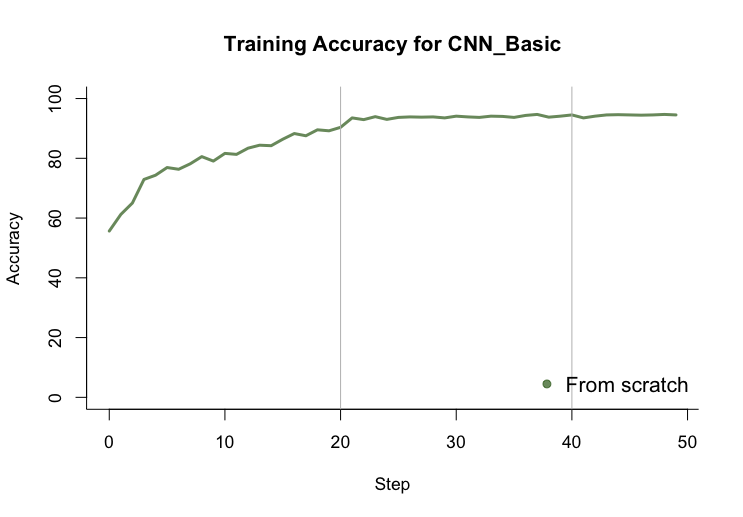
\includegraphics[width=.48\textwidth]{images/chapter5/TrainAccuracy.png}
}
\subfigure{
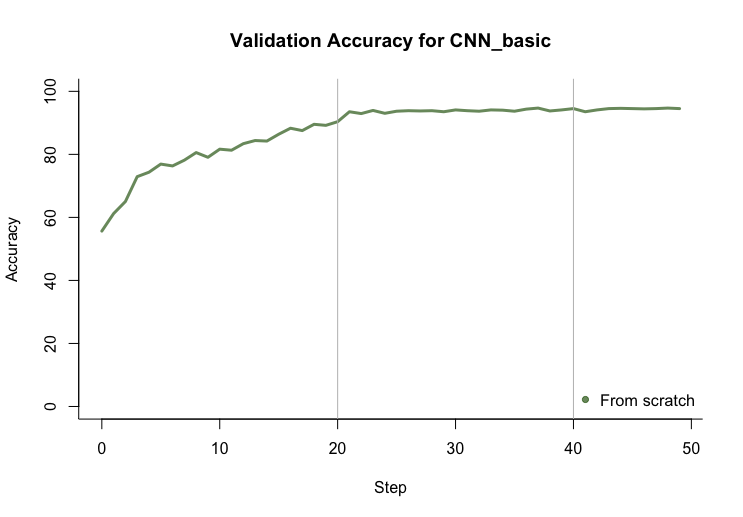
\includegraphics[width=.48\textwidth]{images/chapter5/ValAccuracy.png}
}
\label{fig:cnn-basic}
\end{figure}

\quad

Of course, interpreting this model is very difficult due to it's resizing of the image so early. It could be possible that the model simply learns to label all the images as non-asbestos since the dataset is strongly unbalanced but looking at the confusion matrix in Figure \ref{fig:cnn-basic-cm} shows that the model does not cheat in this way and produces sound looking results. \\


\begin{figure}[!h]
\centering
\caption{Confusion matrix of the CNN\_basic shows that the learning seems to be correct with images seperated into the two classes of asbestos and non-asbestos.}
\subfigure{
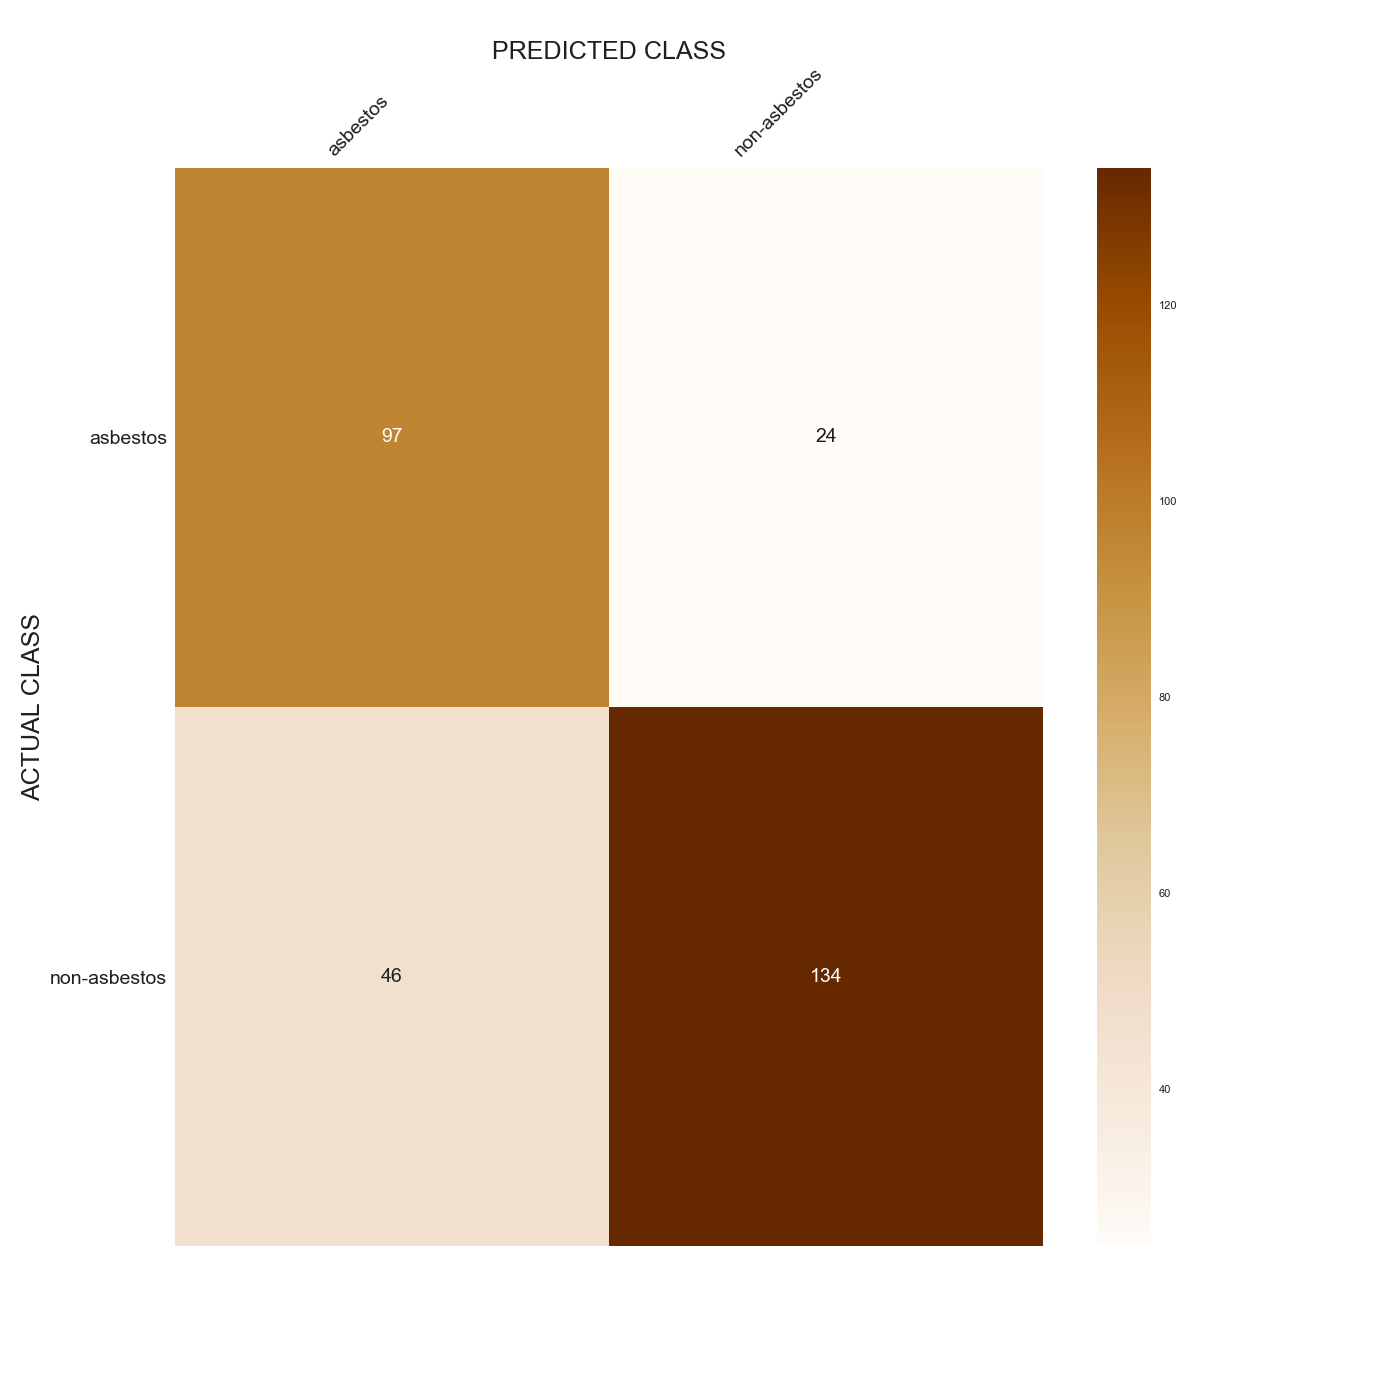
\includegraphics[width=.46\textwidth]{images/chapter5/cnn-basic-cm.png}
}
\label{fig:cnn-basic-cm}
\end{figure}

\quad

From the confusion matrix, we can deduce type I and type II errors. Type I errors are false positives which is equivalent to a false alarm. In case of asbestos, it is better to classify wrongly some structures as asbestos than missing them which would be a type II error or a miss. Recall shows how many positive samples were actually classified as positive which in our case should be as near to 100\% as possible because it brings the type II error in relation to the overall positive samples. Recall is at 80.17\%. Precision on the other hand, shows how many of the predicted positive sample were indeed positive and scores at 67.83\%. Having a low value for Precision is better, than having a low value for recall since it simply means that more samples were classified false as containing asbestos. Rather have a false alarm and recheck than to miss asbestos in samples. \\









%%%%%%%%%%%%%%%%%%%%%%%%%%%%%%%%%%%%%%%%%%%
%%%%%%%%%%%%%%%    ALEXNET    %%%%%%%%%%%%%%%%%%%%
%%%%%%%%%%%%%%%%%%%%%%%%%%%%%%%%%%%%%%%%%%%






\subsection{AlexNet}

AlexNet was optimized with grid search and additionally with SigOpt. With grid search the best accuracy is 81.06\% as seen in table \ref{tbl:alexnet-baseline}. It was achieved with a learning rate of 0.0001 and a learning rate decay of 20. Interestingly the SigOpt also achieved the same accuracy with a learning rate of 0.038984, a momentum of 0.073145 and a weight decay of 0.004074 as seen in table \ref{tbl:alexnet-baseline}. \\



\begin{table*}[!h]
    \ra{1.3}
    \caption{Accuracy (\%) for several learning rates and lr-decays for AlexNet as a baseline.}
    \centering
    \begin{small}
    \textsc{
      \resizebox{0.99\textwidth}{!}{%
      \begin{tabular}{rcclcclcc}
      \toprule 
      & \multicolumn{2}{c}{Learning-Rate decay: 10} && %
        \multicolumn{2}{c}{Learning-Rate decay: 15} && %
        \multicolumn{2}{c}{Learning-Rate decay: 20} \\
      \cmidrule{2-3} \cmidrule{5-6}  \cmidrule{8-9}
      & learning rate & accuracy  && %
        learning rate & accuracy  && %
        learning rate & accuracy  \\ 
      \midrule
      AlexNet        & 0.1 & 59.80\%  &&  0.1 & 59.80\% &&  0.1 & 60.47\% \\
      AlexNet        & 0.05 & 59.80\%  &&  0.05 & 59.80\% && 0.05 & 59.80\% \\
      AlexNet        & 0.01 & 59.80\%  &&  0.01 & 59.80\% &&  0.01 & 59.80\% \\
      AlexNet        & 0.005 & 59.80\%  &&  0.005 & 59.80\% &&  0.005 & 59.80\% \\
      AlexNet        & 0.001 & 74.75\%  &&  0.001 & 77.74\% &&  0.001 & 78.74\% \\
      AlexNet        & 0.0005 & 78.74\%  &&  0.0005 & 80.40\% &&  0.0005 & 76.74\% \\
      AlexNet        & 0.0001 & 74.75\%  &&  0.0001 & 80.07\% &&  \textbf{0.0001} & \textbf{81.06\%} \\
    \bottomrule
    \end{tabular}}
    }
    \end{small}
    %\end{center}
    \vspace{-3.9mm}
    \label{tbl:alexnet-baseline}
\end{table*}

\quad

\subsection{Transfer learning on AlexNet}

When using weights from pre-training on ImageNet, the overall accuracy does get slightly better, although the increase of 0.6645\% is very slim and could be due to chance. In order to assert that pre-training really helps with AlexNet, each model has been run 5 times with the found hyper parameters and the results are averaged as seen in Table \ref{tbl:AlexNetMultiRun}. The delta of both models increased to roughly 1\%. \\


\begin{table}[!h] \centering
\ra{1.3}
\caption{Hyper parameters for Alexnet optimized with SigOpt. First line shows the model trained from scratch and the second line shows the pre-trained model.}
\resizebox{0.99\textwidth}{!}{%
\begin{tabular}{@{}rrrrrrr@{}}
\toprule & learning rate & momentum & weight\_decay & lr-decay & accuracy & $\Delta$ \\
\midrule
AlexNet from scratch    & 0.038498 & 0.073146 &  0.004074 & 20 & 81.0631\%  &         \\
\textbf{AlexNet pre-trained}    & \textbf{0.034288} & \textbf{0.409378} &  \textbf{0.005959} & \textbf{20} & \textbf{81.7276\%}  & \textbf{+0.6645}\\
\bottomrule
\end{tabular}}
\label{tbl:AlexNetBaseline}
\end{table}

\quad

\begin{table}[!h] \centering
\ra{1.3}
\caption{The Alexnet architecture was run 5 times with the found hyperparameters and averaged across the runs. Aditionally the Adam optimizer is used instead of weight and lr-decay.}
\resizebox{0.99\textwidth}{!}{%
\begin{tabular}{@{}rrrrrrr@{}}
\toprule & learning rate & momentum & weight\_decay & lr-decay & accuracy & $\Delta$ \\
\midrule
AlexNet     from scratch    & 0.038498 & 0.073146 &  0.004074 & 20 & 78.61$\pm$1.16  & -     \\
AlexNet     pre-trained    & 0.034288 & 0.409378 &  0.005959 & 20 & 79.67$\pm$1.08  & - \\
AlexNet from scratch (Adam Optimizer) & 0.038498 & Adam & Adam & 20 & 59.80$\pm$0.0 & \\
\bottomrule
\end{tabular}}
\label{tbl:AlexNetMultiRun}
\end{table}

\quad

In Figure \ref{fig:alexnet-graph} we see the training and validation accuracies plotted over epochs. It can be observed that convergence is not faster with pre-training than without pre-training. Both final accuracies are almost identical. The gray vertical lines separate the graph into segments with different learning rates. So the learning rate decay happens a first time at epoch 20 and a second time at epoch 40. Convergence can be easily observed when the validation accuracy does not change anymore. Another important thing to notice is that validation and training accuracies are quite near to each other. This means that during training no severe overfitting occurred and that the validation set and train set are indeed very representative of each other. Since the final accuracy is also very near to these values it is save to say that validation and train sets are good representations of the test set. \\


\begin{figure}[!h]
\centering
\caption{No clear difference can be observed between the pre-trained AlexNet and the not pre-trained AlexNet. Both converge roughly equally and reach almost the same final accuracy.}
\subfigure{
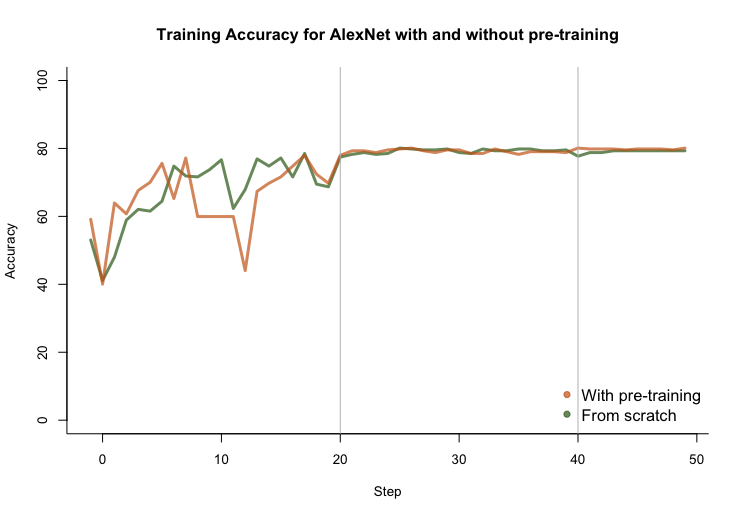
\includegraphics[width=.46\textwidth]{images/chapter5/TL/AlexNet/TA-AlexNet.png}
}
\subfigure{
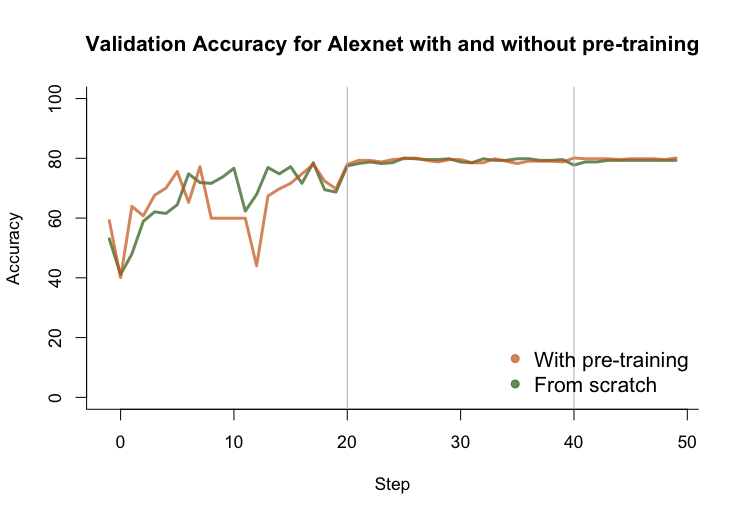
\includegraphics[width=.46\textwidth]{images/chapter5/TL/AlexNet/VA-AlexNet.png}
}
\label{fig:alexnet-graph}
\end{figure}

\quad

In Figure \ref{fig:alexnet-cm} the confusion matrix of the final test set is shown for both models (pre-trainend and non pre-trained). \\


\begin{figure}[!h]
\centering
\caption{Confusion matrix from the model trained from scratch on the left side, and the model with pre-trained weights on the right.}
\subfigure{
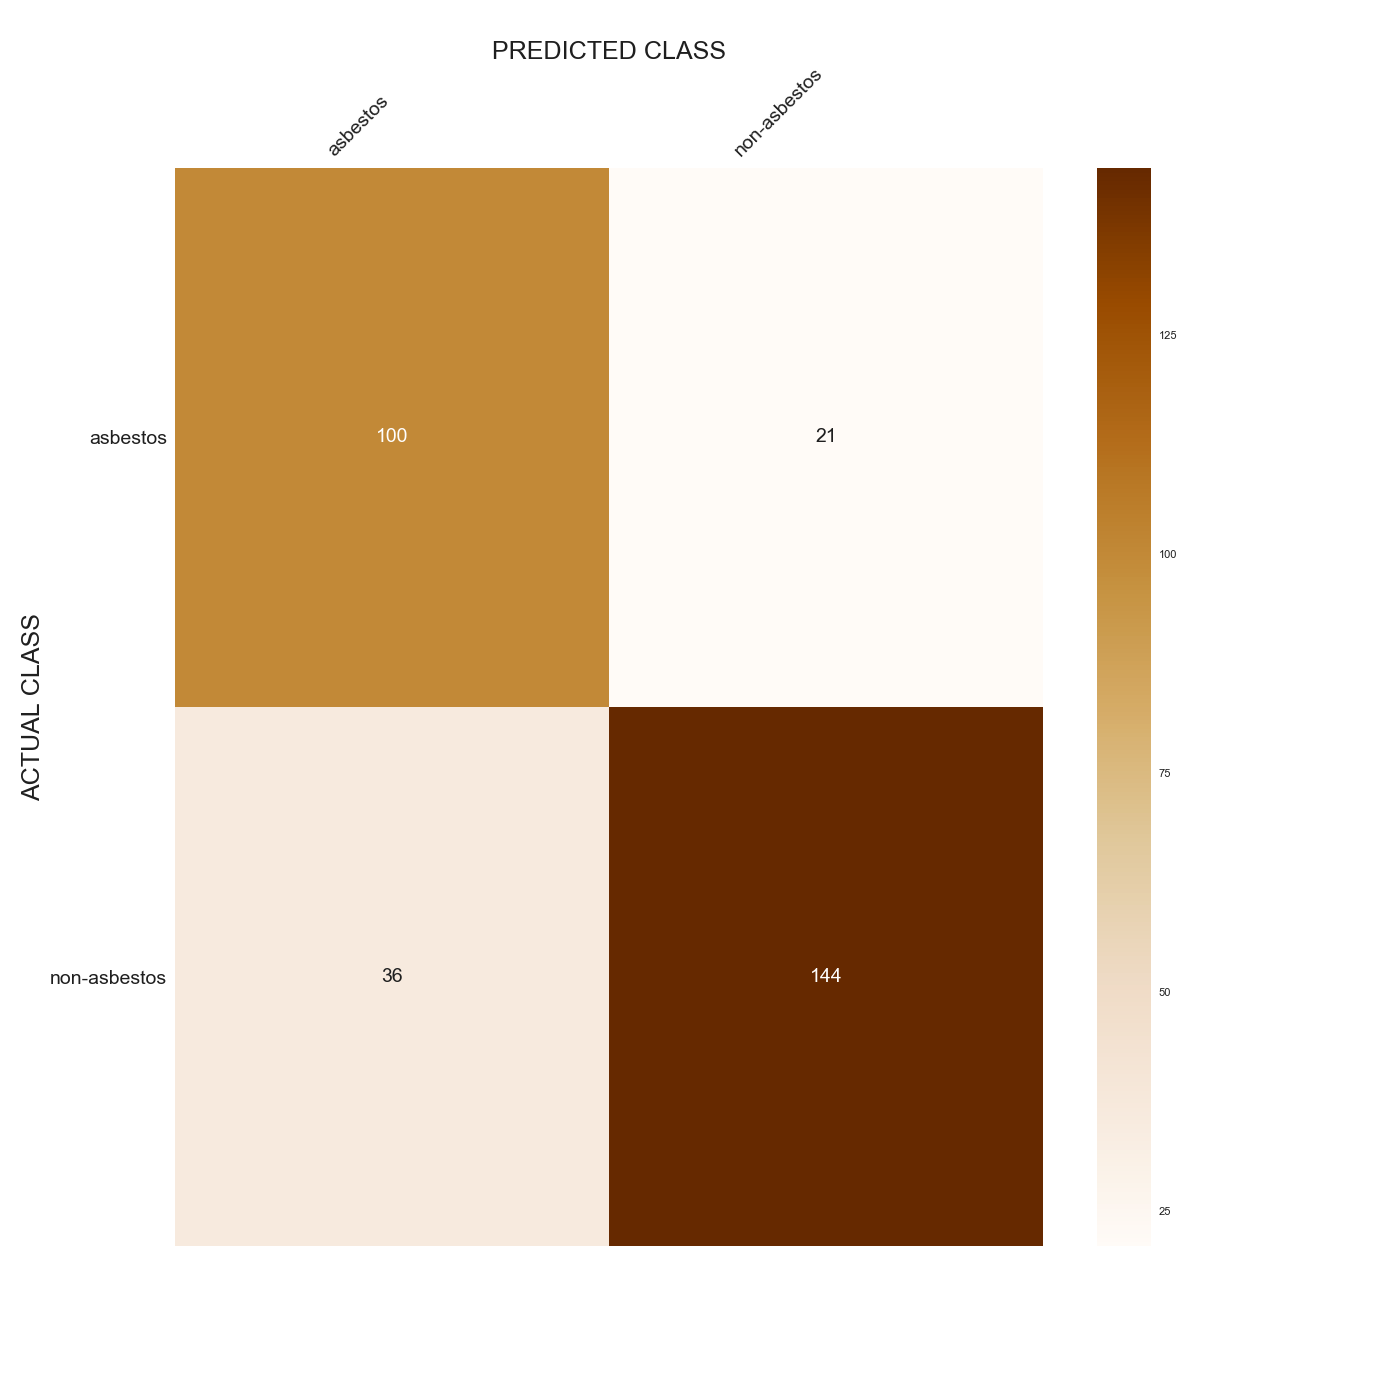
\includegraphics[width=.46\textwidth]{images/chapter5/TL/AlexNet/cm-alexnet.png}
}
\subfigure{
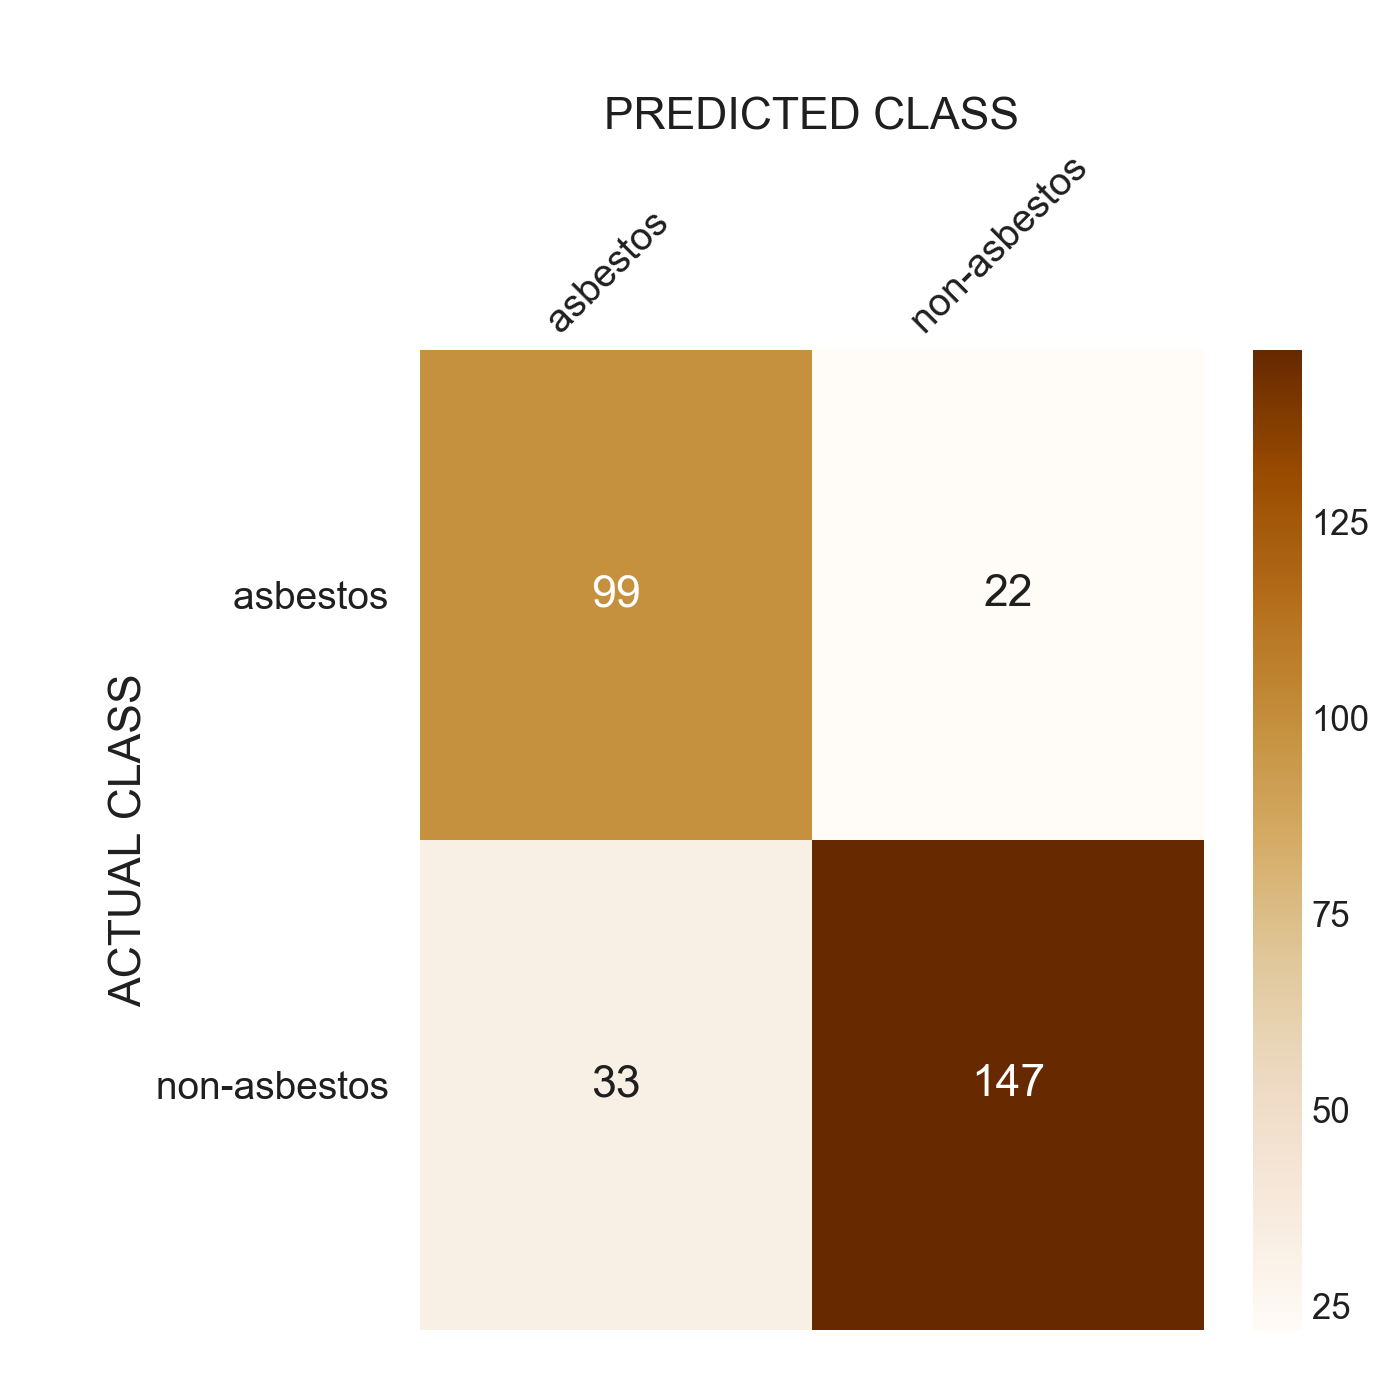
\includegraphics[width=.46\textwidth]{images/chapter5/TL/AlexNet/cm-alexnet-pre.png}
}
\label{fig:alexnet-cm}
\end{figure}

\quad







%%%%%%%%%%%%%%%%%%%%%%%%%%%%%%%%%%%%%%%%%%%
%%%%%%%%%%%%%%%%    VGG    %%%%%%%%%%%%%%%%%%%%%
%%%%%%%%%%%%%%%%%%%%%%%%%%%%%%%%%%%%%%%%%%%


\section{VGG}

For the following VGG architectures, the hyperparameter optimization was done with SigOpt. Every architecture was performed with and without batch normalization as well as with and without pre-training. Table \ref{tbl:VGG_overview} summarizes the results for the VGG architectures with the common depths of 11, 13 and 16. These are all the best achieved values in one run only. \\


\begin{table}[!h] \centering
\ra{1.3}
\caption{Hyper parameters for VGG11, VGG13 and VGG16 with and without batch normalization (bn) optimized with SigOpt. First row of each grouping shows training the architecture from scratch. Second row of each grouping shows training with pre-trained weights from ImageNet}
\resizebox{0.99\textwidth}{!}{%
\begin{tabular}{@{}rrrrrrr@{}}
\toprule & learning rate & momentum & weight\_decay & lr-decay & accuracy & $\Delta$ \\
\midrule
VGG11 from scratch		& 0.026981 & 0.743190 & 0.01 & 20 & 80.7309\%  &         \\
VGG11 pre-trained		& 0.006787 & 0.696714 & 0.01 & 20 & 88.0399\%  & +7.309 \\
\midrule
VGG11\_bn  from scratch	&     0.059343 & 0.120718 &  0.009362 & 20 & 81.0631\%  &         \\
\textbf{VGG11\_bn pre-trained}	& \textbf{0.022571} & \textbf{0.383537} &  \textbf{0.001733} & \textbf{20} &  \textbf{89.7010\%} & \textbf{+8.6379} \\
\midrule
VGG13 from scratch		& 0.033844 & 0.257538 &  0.01 & 20 & 81.0631\%  &         \\
VGG13 pre-trained    	& 0.020012 & 0.193932 & 0.01 & 20 & 88.7043\%  & +7.6412 \\
\midrule
VGG13\_bn from scratch    			& 0.054173 & 0.643504 &  0.003223 & 20 & 81.7276\%  &         \\
\textbf{VGG13\_bn  pre-trained}    &  \textbf{0.093533} & \textbf{0.041074} &  \textbf{0.009734} & \textbf{20} & \textbf{90.3655\%}  & \textbf{+8.6379} \\
\midrule
VGG16 from scratch   	& 0.019590 & 0.383297 &  0.00001 & 20 & 81.7276\%  &         \\
\textbf{VGG16 pre-trained}    	& \textbf{0.009735} & \textbf{0.529937} & \textbf{0.01} & \textbf{20} & \textbf{90.6977\%}  & \textbf{+8.9701} \\
\midrule
VGG16\_bn from scratch	&     0.031702 & 0.370868 &  0.006288 & 20 & 83.0565\%  &         \\
VGG16\_bn pre-trained		&     0.083995 & 0.242109 &  0.002634 & 20 & 89.0366\%  & +5.9801 \\
\bottomrule
\end{tabular}}
\label{tbl:VGG_overview}
\end{table}

\quad

It can be seen that transfer learning helps in every single case and yields better performance by roughly additional 8\%. Also VGG performs generally better with batch normalization with one exception for VGG16 with pre-trained weights. This architecture outperformed its batch norm counterpart by 1.66\% which could be purely by chance. VGG13 with batch normalization seems to perform very well, although by a very small margin, since it is also less complex than VGG16, it will be used for further investigation. First, it is run three times with the found hyper parameters and then averaged as seen in Table \ref{tbl:VGG_averaged}. Since the values mentioned in Table \ref{tbl:VGG_overview} are the best values from 30 runs, it does not surprise that they are higher than the averaged values from Table \ref{tbl:VGG_averaged}. \\


\begin{table}[!h] \centering
\ra{1.3}
\caption{Running the best VGG architecture three times with the found hyperparameters and averaging across the total of runs. }
\resizebox{0.99\textwidth}{!}{%
\begin{tabular}{@{}rrrrrrr@{}}
\toprule & learning rate & momentum & weight\_decay & lr-decay & accuracy & $\Delta$ \\
\midrule
VGG13\_bn from scratch	& 0.054173 	& 0.643504 	& 0.003223 	& 20 	& 81.0631\% $\pm$ 0.5425 &         \\
VGG13\_bn pre-trained		& 0.093533 	& 0.041074 	& 0.009734 	& 20 	& 88.0399\% $\pm$ 0.7176 & +6.9768\\
\bottomrule
\end{tabular}}
\label{tbl:VGG_averaged}
\end{table}

\quad

Looking at the training and validation graphs in Figure \ref{fig:vgg13-graph} a very similar behavior can be observed as in the previous graphs of the AlexNet architectures. Training accuracy is overfitting with the pre-trained model very quickly, convergence happens within the first 20 epochs, while training from scratch needs roughly 30 epochs to converge and never catches up with the pre-trained model. For the validation graph, convergence happens for both models shortly after 20 epochs and the validation accuracy is better with pre-trained weights (87.98\%) than from scratch (79.79\%). Both values are very near the actual values obtained in the test set which again confirms the hypothesis that the validation set does represent the test set very well. \\


\begin{figure}[!h]
\centering
\caption{Training and validation graphs for VGG13 once with pre-trained weights from ImageNet (orange) and once trained from scratch (green)}
\subfigure{
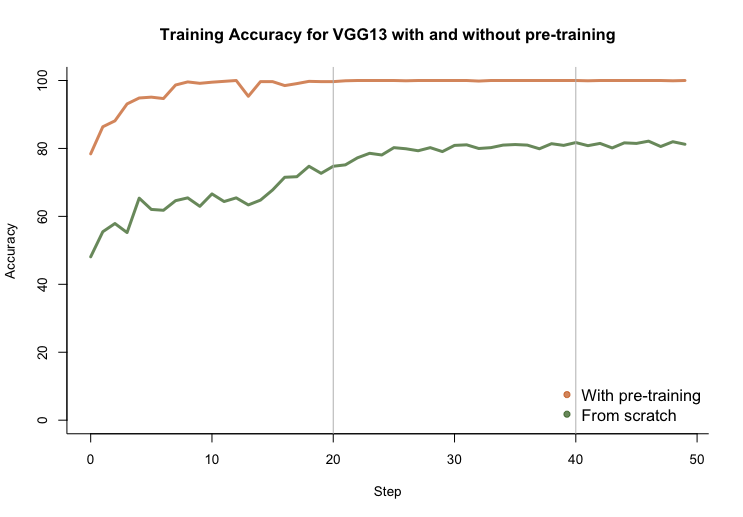
\includegraphics[width=.46\textwidth]{images/chapter5/TL/VGG13/TA-vgg13.png}
}
\subfigure{
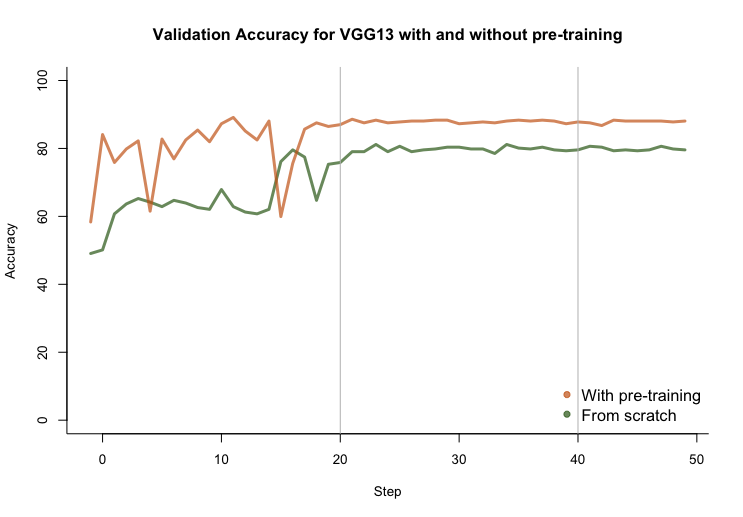
\includegraphics[width=.46\textwidth]{images/chapter5/TL/VGG13/VA-vgg13.png}
}
\label{fig:vgg13-graph}
\end{figure}

\quad

\subsection{VGG visualization}

In order to shed some light into what is going on, visualizing the CNN layers can show what kind of input images activate a specific filter and thus lead to a certain classification. Several hundred visualizations were checked at different layers for VGG13\_bn with and without transfer learning. In Figure \ref{fig:vgg13_pretrained_filters} 16 interesting layer activations from the pretrained model are shown. Filters that resembled rocks, background or fiber-like structures were selected from 4 different layers. \\


\begin{figure}[!h]
\centering
\caption{Each line represents one convolution layer in the VGG13\_bn pre-trained architecture in ascending order. Four interesting activations are shown per layer starting at layer 2, layer 4, layer 7 and layer 9.}
\subfigure{
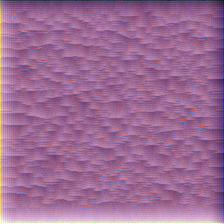
\includegraphics[width=.23\textwidth]{images/chapter5/vgg13-bn-pre/l3-f0.jpg}
}
\subfigure{
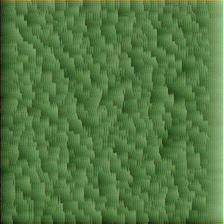
\includegraphics[width=.23\textwidth]{images/chapter5/vgg13-bn-pre/l3-f1.jpg}
}
\subfigure{

\includegraphics[width=.23\textwidth]{images/chapter5/vgg13-bn-pre/l3-f2.jpg}
}
\subfigure{
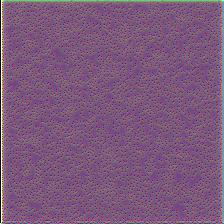
\includegraphics[width=.23\textwidth]{images/chapter5/vgg13-bn-pre/l3-f3.jpg}
}

\subfigure{

\includegraphics[width=.23\textwidth]{images/chapter5/vgg13-bn-pre/l10-f0.jpg}
}
\subfigure{

\includegraphics[width=.23\textwidth]{images/chapter5/vgg13-bn-pre/l10-f1.jpg}
}
\subfigure{
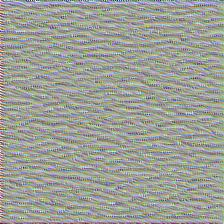
\includegraphics[width=.23\textwidth]{images/chapter5/vgg13-bn-pre/l10-f2.jpg}
}
\subfigure{
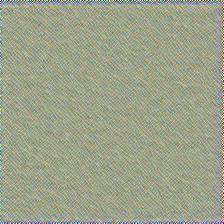
\includegraphics[width=.23\textwidth]{images/chapter5/vgg13-bn-pre/l10-f3.jpg}
}

\subfigure{

\includegraphics[width=.23\textwidth]{images/chapter5/vgg13-bn-pre/l21-f0.jpg}
}
\subfigure{

\includegraphics[width=.23\textwidth]{images/chapter5/vgg13-bn-pre/l21-f1.jpg}
}
\subfigure{

\includegraphics[width=.23\textwidth]{images/chapter5/vgg13-bn-pre/l21-f2.jpg}
}
\subfigure{

\includegraphics[width=.23\textwidth]{images/chapter5/vgg13-bn-pre/l21-f3.jpg}
}

\subfigure{

\includegraphics[width=.23\textwidth]{images/chapter5/vgg13-bn-pre/l28-f0.jpg}
}
\subfigure{
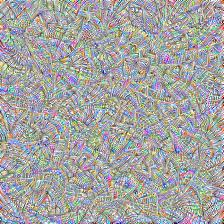
\includegraphics[width=.23\textwidth]{images/chapter5/vgg13-bn-pre/l28-f1.jpg}
}
\subfigure{

\includegraphics[width=.23\textwidth]{images/chapter5/vgg13-bn-pre/l28-f2.jpg}
}
\subfigure{

\includegraphics[width=.23\textwidth]{images/chapter5/vgg13-bn-pre/l28-f3.jpg}
}
\label{fig:vgg13_pretrained_filters}
\end{figure}

\quad

It can be very well observed that with increasing depth of the network more complex patterns are learned. In Figure \ref{fig:vgg13_app_pretrained_filters_a}, Figure \ref{fig:vgg13_app_pretrained_filters_b} and Figure \ref{fig:vgg13_app_pretrained_filters_c} in the Appendix, four images are shown for every layer in the architecture. The first layer learns only to spot plain colors, but already the second layer starts to look for vertical and horizontal rock-like patterns, as seen in Figure \ref{fig:vgg13_fromscratch_filters}. Some of the filters don't resemble anything from the training set but still have a high degree of pattern. These patterns were transferred over from ImageNet and adapted through 50 epochs of learning. Figure \ref{fig:vgg13_fromscratch_filters} shows four layers of the pre-trained VGG13 architectue. \\


\begin{figure}[!h]
\centering
\caption{Each line represents one convolution layer in the VGG13\_bn architecture which was trained from scratch in ascending order. Four interesting activations are shown per layer starting at layer 2, layer 4, layer 7 and layer 9.}
\subfigure{
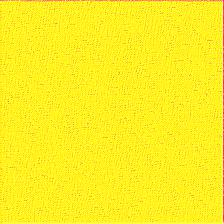
\includegraphics[width=.23\textwidth]{images/chapter5/vgg13-bn/l3-f0.jpg}
}
\subfigure{
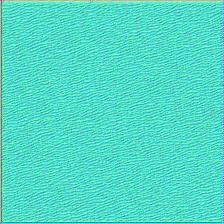
\includegraphics[width=.23\textwidth]{images/chapter5/vgg13-bn/l3-f1.jpg}
}
\subfigure{

\includegraphics[width=.23\textwidth]{images/chapter5/vgg13-bn/l3-f2.jpg}
}
\subfigure{
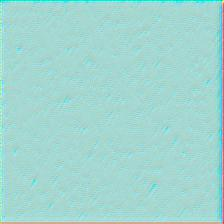
\includegraphics[width=.23\textwidth]{images/chapter5/vgg13-bn/l3-f3.jpg}
}

\subfigure{
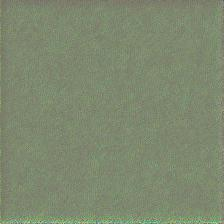
\includegraphics[width=.23\textwidth]{images/chapter5/vgg13-bn/l10-f0.jpg}
}
\subfigure{

\includegraphics[width=.23\textwidth]{images/chapter5/vgg13-bn/l10-f1.jpg}
}
\subfigure{
\includegraphics[width=.23\textwidth]{images/chapter5/vgg13-bn/l10-f2.jpg}
}
\subfigure{
\includegraphics[width=.23\textwidth]{images/chapter5/vgg13-bn/l10-f3.jpg}
}

\subfigure{
\includegraphics[width=.23\textwidth]{images/chapter5/vgg13-bn/l21-f0.jpg}
}
\subfigure{
\includegraphics[width=.23\textwidth]{images/chapter5/vgg13-bn/l21-f1.jpg}
}
\subfigure{
\includegraphics[width=.23\textwidth]{images/chapter5/vgg13-bn/l21-f2.jpg}
}
\subfigure{
\includegraphics[width=.23\textwidth]{images/chapter5/vgg13-bn/l21-f3.jpg}
}

\subfigure{
\includegraphics[width=.23\textwidth]{images/chapter5/vgg13-bn/l28-f0.jpg}
}
\subfigure{
\includegraphics[width=.23\textwidth]{images/chapter5/vgg13-bn/l28-f1.jpg}
}
\subfigure{
\includegraphics[width=.23\textwidth]{images/chapter5/vgg13-bn/l28-f2.jpg}
}
\subfigure{
\includegraphics[width=.23\textwidth]{images/chapter5/vgg13-bn/l28-f3.jpg}
}
\label{fig:vgg13_fromscratch_filters}
\end{figure}

\quad

It is very interesting to observe that no complex patterns can be found in these layer activations. Instead, there is a lot of noise in the images. Although rock like structures could be interpreted into these visualizations, fiber like structures are missing completely.

Applying Grad-CAM and heatmap visualizations can show important regions of the image that correspond to a certain classification. These areas are colored in deep red to orange, whereas areas that did not contribute are colored in blue to violet. Figure \ref{fig:vgg13_pre_heatmap} shows two Gad-CAM visualizations from different layers. In the first row the second convolution layer is shown with the network recognizing rather fine-grained regions detected by the low-level feature maps. The second row shows the last convolution layer where high-level feature maps are captured. \\


\begin{figure}[!h]
\centering
\caption{Grad-Cam and heatmap visualizations are shown for the pre-trained architectures for layers 3 and 31}
\subfigure{
\includegraphics[width=.25\textwidth]{images/chapter5/vgg13-bn-pre/7-Cam-Grayscale.png}
}
\subfigure{
\includegraphics[width=.25\textwidth]{images/chapter5/vgg13-bn-pre/7-Cam-Heatmap.png}
}
\subfigure{
\includegraphics[width=.25\textwidth]{images/chapter5/vgg13-bn-pre/7-Cam-Image.png}
}

\subfigure{
\includegraphics[width=.25\textwidth]{images/chapter5/vgg13-bn-pre/31-Cam-Grayscale.png}
}
\subfigure{
\includegraphics[width=.25\textwidth]{images/chapter5/vgg13-bn-pre/31-Cam-Heatmap.png}
}
\subfigure{
\includegraphics[width=.25\textwidth]{images/chapter5/vgg13-bn-pre/31-Cam-Image.png}
}
\label{fig:vgg13_pre_heatmap}
\end{figure}

\quad

In Figure \ref{fig:vgg13_heatmap}, the same Grad-CAM visualizations are shown at the same layers for the model trained from scratch. It can be easily seen that although the low-level features are still similar the last convolution layer yields completely different results. \\


\begin{figure}[!h]
\centering
\caption{Grad-Cam and heatmap visualizations for the model trained from scratch. Layers 3 and 31 are shown.}
\subfigure{
\includegraphics[width=.25\textwidth]{images/chapter5/vgg13-bn/7-Cam-Grayscale.png}
}
\subfigure{
\includegraphics[width=.25\textwidth]{images/chapter5/vgg13-bn/7-Cam-Heatmap.png}
}
\subfigure{
\includegraphics[width=.25\textwidth]{images/chapter5/vgg13-bn/7-Cam-Image.png}
}


\subfigure{
\includegraphics[width=.25\textwidth]{images/chapter5/vgg13-bn/31-Cam-Grayscale.png}
}
\subfigure{
\includegraphics[width=.25\textwidth]{images/chapter5/vgg13-bn/31-Cam-Heatmap.png}
}
\subfigure{
\includegraphics[width=.25\textwidth]{images/chapter5/vgg13-bn/31-Cam-Image.png}
}
\label{fig:vgg13_heatmap}
\end{figure}

\quad









%%%%%%%%%%%%%%%%%%%%%%%%%%%%%%%%%%%%%%%%%%%
%%%%%%%%%%%%%%%%%    RESNET    %%%%%%%%%%%%%%%%%%%
%%%%%%%%%%%%%%%%%%%%%%%%%%%%%%%%%%%%%%%%%%%




\section{ResNet}

ResNet18 and ResNet34 were both optimized with SigOpt only. For each hyper parameter 10 runs were conducted summing up to 30 runs. It was used for training the architecture from scratch and with pre-trained weights. Table \ref{tbl:ResNet18_overview} shows a summary of the optimization process with the best accuracies and the delta between the pre-trained model and the model trained from scratch. \\


\begin{table}[!h] \centering
\ra{1.3}
\caption{Hyper parameters for ResNet18 and ResNet34 optimized with SigOpt. First row shows hyperparameters training the architecture from scratch. Second row used pre-trained weights from ImageNet}
\resizebox{0.99\textwidth}{!}{%
\begin{tabular}{@{}rrrrrrr@{}}
\toprule & learning rate & momentum & weight\_decay & lr-decay & accuracy & $\Delta$ \\
\midrule
ResNet18 from scratch    & 0.033678 & 0.952630 &  0.007518 & 20 & 83.0565\%  &         \\
\textbf{ResNet18 pre-trained}    & \textbf{0.039918} & \textbf{0.170826} & \textbf{0.001980} & \textbf{20} & \textbf{88.0399\%}  & \textbf{+4.9834}\\
\midrule
ResNet34 from scratch    & 0.040323 & 0.141704 &  0.004044 & 20 & 83.0565\%  &         \\
ResNet34 pre-trained    & 0.060848 & 0.460187 &  0.000537 & 20 & 87.0431\%  & +3.9866\\
\bottomrule
\end{tabular}}
\label{tbl:ResNet18_overview}
\end{table}

\quad

ResNet18 and ResNet34 perform equally well when trained form scratch but differ slightly when pre-trained weights from ImageNet are used. The increased gain from transfer learning for ResNet18 is thus higher and since it has less parameters, it is the preferred architecture to be further evaluated.\\

The graphs in Figure \ref{fig:resnet18-graph} show clearly that training converged much faster for the model with pre-trained weights. After only a few epochs it reached convergence while the model without pre-trained weights had to catch up over many epochs. Both models overfit strongly to the training data and yield lower results in the validation and test sets. Interestingly the validation accuracy of the model trained from scratch starts to decrease around epoch 30 although training accuracy still rises. This is considered bad and is also reflected in the final accuracies where the model without transfer learning scores around 5\% lower. \\


\begin{figure}[!h]
\centering
\caption{Training and validation graphs for ResNet18 once with pre-trained weights from ImageNet and once trained from scratch.}
\subfigure{
\includegraphics[width=.46\textwidth]{images/chapter5/TL/ResNet18/TA-ResNet18.png}
}
\subfigure{
\includegraphics[width=.46\textwidth]{images/chapter5/TL/ResNet18/VA-ResNet18.png}
}
\label{fig:resnet18-graph}
\end{figure}

\quad

With the confusion matrix in Figure \ref{fig:resnet18-cm} we can see that the learning did not take any shortcuts and that the distinction between images with asbestos fibers and images without were clearly separated to some extent that is reflected in the overall accuracy reached. The Precision and Recall for the model trained from scratch are 77.78\% and 80.99\%, respectively. For the model with pre-trained weight, Precision and Recall are much better with 83.47\% and 87.60\%, respectively. \\


\begin{figure}[!h]
\centering
\caption{On the left: confusion matrix from model trained from scratch. On the right trained with transfer learning applied.}
\subfigure{
\includegraphics[width=.46\textwidth]{images/chapter5/TL/ResNet18/cm-resnet18.png}
}
\subfigure{
\includegraphics[width=.46\textwidth]{images/chapter5/TL/ResNet18/cm-resnet18-pre.png}
}
\label{fig:resnet18-cm}
\end{figure}

\quad









%%%%%%%%%%%%%%%%%%%%%%%%%%%%%%%%%%%%%%%%%%%
%%%%%%%%%%%%%%%    DENSENET121    %%%%%%%%%%%%%%%%%
%%%%%%%%%%%%%%%%%%%%%%%%%%%%%%%%%%%%%%%%%%%



\section{Densenet121}

Densenet121 and Densenet169 were both optimized with SigOpt only. For each hyper parameter 10 runs were conducted summing up to 30 runs. It was used for training the architecture from scratch and with pre-trained weights. Table \ref{tbl:Densenet121_overview} shows a summary of the optimization process with the best accuracies and the delta between the pre-trained model and the model trained from scratch.\\


\begin{table}[!h] \centering
\ra{1.3}
\caption{Hyper parameters for densenet121 optimized with SigOpt. First row shows hyperparameters training the architecture from scratch. Second row used pre-trained weights from ImageNet}
\resizebox{0.99\textwidth}{!}{%
\begin{tabular}{@{}rrrrrrr@{}}
\toprule & learning rate & momentum & weight\_decay & lr-decay & accuracy & $\Delta$ \\
\midrule
Densenet121 from scratch    & 0.035925 & 0.057618 &  0.009241 & 20 & 86.0465\%  &         \\
\textbf{Densenet121 pre-trained}    & \textbf{0.018489}     & \textbf{0.369998} &  \textbf{0.004963} & \textbf{20} & \textbf{88.3721\%}  & \textbf{+2.3256} \\
\midrule
Densenet169 from scratch    & 0.005812 & 0.777249 & 0.006999  & 20 & 85.3821\%  &         \\
Densenet169 pre-trained    & 0.006347 & 0.447591 & 0.005180 & 20 & 89.3688\%  & +3.9867\\
\bottomrule
\end{tabular}}
\label{tbl:Densenet121_overview}
\end{table}

\quad

As already seen in the previous comparisons of VGG and ResNet architectues, the parameter size does not seem to play a role in this specific task. If the model is trained from scratch, Densenet121 achieves slightly higher accuracies than Densenet161. The opposite is true for the model trained with transfer learning where Densenet169 performs slightly better. Since the difference is very small Densenet121 is preferred for further investigation over the deeper Densenet169 architecture.

The graphs in Figure \ref{fig:densenet121-graph} show again a very similar and already known behavior. Convergence happens much faster with the pre-trained model. Training overfits strongly to the training data. Validation accuracies are similar to the test accuracies. Since the confusion materices for the Densenet121 architecture look almost identical as in VGG13 and ResNet18 I decided to omit them for brevity. \\


\begin{figure}[!h]
\centering
\caption{Training and validation graphs for Densenet121 once with pre-trained weights from ImageNet and once trained from scratch.}
\subfigure{
\includegraphics[width=.46\textwidth]{images/chapter5/TL/Densenet121/TA-densenet121.png}
}
\subfigure{
\includegraphics[width=.46\textwidth]{images/chapter5/TL/Densenet121/VA-densenet121.png}
}
\label{fig:densenet121-graph}
\end{figure}

\quad







%%%%%%%%%%%%%%%%%%%%%%%%%%%%%%%%%%%%%%%%%%%
%%%%%%%%%%%%%%%    INCEPTIONv3   %%%%%%%%%%%%%%%%%%
%%%%%%%%%%%%%%%%%%%%%%%%%%%%%%%%%%%%%%%%%%%



\section{Inception}


Hyperparameter optimization for Inception v3 was done with SigOpt and for both variants, training from scratch and training with pre-trained weights from ImageNet.

Inception v3 was optimized with SigOpt only. For each hyper parameter 10 runs were conducted summing up to 30 runs. It was used for training the architecture from scratch and with pre-trained weights. Table \ref{tbl:Inceptionv3_overview} shows a summary of the optimization process with the best accuracies and the delta between the pre-trained model and the model trained from scratch. \\


\begin{table}[!h] \centering
\ra{1.3}
\caption{Hyper parameters for Inception v3 optimized with SigOpt. First row shows hyperparameters training the architecture from scratch. Second row used pre-trained weights from ImageNet}
\resizebox{0.99\textwidth}{!}{%
\begin{tabular}{@{}rrrrrrr@{}}
\toprule & learning rate & momentum & weight\_decay & lr-decay & accuracy & $\Delta$ \\
\midrule
Inception v3 from scratch    & 0.070046 & 0.910505 & 0.006943 & 20 & 83.3887\%  &         \\
\textbf{Inception v3 pre-trained}    & \textbf{0.029269} & \textbf{0.0} & \textbf{0.006320} & \textbf{20} & \textbf{88.7043\%}  & \textbf{+5.3156} \\
\bottomrule
\end{tabular}}
\label{tbl:Inceptionv3_overview}
\end{table}

\quad

The same behaviour is seen again with Inception v3 as with the previous architectures. Using pre-trained weights from ImageNet can help the model converge faster and find a better solution as seen in Figure \ref{fig:inception-graph}. The confusion matrices have been omitted since they look almost identical to the previous confusion matrices from VGG13 in Figure \ref{fig:vgg13_heatmap} and ResNet18 in Figure \ref{fig:resnet18-cm} \\


\begin{figure}[!h]
\centering
\caption{Training and validation graphs for Inception v3 once with pre-trained weights from ImageNet and once trained from scratch.}
\subfigure{
\includegraphics[width=.46\textwidth]{images/chapter5/TL/inception/TA-inception.png}
}
\subfigure{
\includegraphics[width=.46\textwidth]{images/chapter5/TL/inception/VA-inception.png}
}
\label{fig:inception-graph}
\end{figure}

\quad

\section{Conclusion on Transfer Learning}

Using pre-trained weights from ImageNet increased accuracy of every single run performed on the above mentioned architectures. Apparently, learning feature representations from a broad dataset like the ImageNet does indeed transfer very well to different target domains. These findings align perfectly well with other research done on cross-domain transfer learning. By average the models get a 5.18\% boost from pre-training on ImageNet with Alexnet having the smallest increase of only 0.66\% while VGG16 had the biggest increase of 8.97\%. Table \ref{tbl:transferlearning_overview} summarizes the most relevant findings on transfer learning.

\begin{table}[!h] \centering
\ra{1.3}
\caption{Summary of transfer learning results. Only relevant results are shown that are used in the next chapter.}
\resizebox{0.99\textwidth}{!}{%
\begin{tabular}{@{}rrrrrrr@{}}
\toprule & learning rate & momentum & weight\_decay & lr-decay & accuracy & $\Delta$ \\
\midrule
VGG13\_bn from scratch    			& 0.054173 & 0.643504 &  0.003223 & 20 & 81.7276\%  &         \\
\textbf{VGG13\_bn pre-trained} 	& \textbf{0.093533} & \textbf{0.041074} & \textbf{0.009734} & \textbf{20} & \textbf{90.3655\%}  & \textbf{+8.6379} \\
\midrule
ResNet18 from scratch    & 0.033678 & 0.952630 &  0.007518 & 20 & 83.0565\%  &         \\
\textbf{ResNet18 pre-trained}    & \textbf{0.039918} & \textbf{0.170826} & \textbf{0.001980} & \textbf{20} & \textbf{88.0399\%}  & \textbf{+4.9834}\\
\midrule
Densenet121 from scratch    & 0.035925 & 0.057618 &  0.009241 & 20 & 86.0465\%  &         \\
\textbf{Densenet121 pre-trained}    & \textbf{0.018489}     & \textbf{0.369998} &  \textbf{0.004963} & \textbf{20} & \textbf{88.3721\%}  & \textbf{+2.3256} \\
\midrule
Inception v3 from scratch    & 0.070046 & 0.910505 & 0.006943 & 20 & 83.3887\%  &         \\
\textbf{Inception v3 pre-trained}    & \textbf{0.029269} & \textbf{0.0} & \textbf{0.006320} & \textbf{20} & \textbf{88.7043\%}  & \textbf{+5.3156} \\
\bottomrule
\end{tabular}}
\label{tbl:transferlearning_overview}
\end{table}

\quad

Overfitting was mainly a problem with the pre-trained model since it converged so much faster than the same model trained from scratch. Sometimes the model without pre-training was able to somehow catch up with the pre-trained counterpart on the training set, but never on the test set. Overfitting is nontheless a big problem from both variant and needs to be addressed by cropping and resizing differently and by introducing some randomness, which could be as simple as randomly flipping and rotating the images before feeding them to the model.

At first it was very surprising that learning from scratch never caught up with the models using transfer learning from ImageNet. I was certain that given enough epochs and different runs the models from scratch should find at least equally suited feature mappings with random initialization of weights. But visualizing  some of the filters quickly made it clear that learning from scratch  with the provided dataset doesn't create elaborate feature mappings as seen from ImageNet. I argue that although the vast majority of feature mappings are absolutely useless for the asbestos classification, some feature mappings of e.g. grass or hair might be similar enough for the filter to activate maximally. Since the asbestos task is only a binary classification few of these filters are enough to predict asbestos with a high accuracy. These elaborate feature mappings are not able to be created from scratch with a dataset of only a few hundred, partially wrongly labeled images, thus the model trained from scratch never reaches the accuracy of the pre-trained model. Therefore I conclude for this chapter that transfer learning is invaluable for this task even though the source domain and target domain are very far apart.


\chapter{Evaluation on other Techniques}

This chapter will go through some other techniques that could prove to be valuable for the asbestos dataset like the training size of the dataset, different cropping methods, different image augmentations and architectures that have been altered to better meet the underlying tasks' demands.

\section{Evaluation Of Overall Number Of Parameters in VGG13}

Here I want to understand how the overall number of parameters affects the performance of the network. VGG13 was built primarily for the ImageNet Challenge and probably is too big for a task like the asbestos detection. In a first step I will try to reduce the fully connected layers since they  contribute to the complexity of the model the most. I will gradually reduce the number of parameters in the last 3 layers and compare the performance by averaging over 3 runs. Table XXX shows the results.

\begin{table}[h] \centering
\ra{1.3}
\caption{Variations in the last 3 fully connected layers of the VGG13 architecture. They were all performed with Batch Normalization. The last columne shows how much parameters remain in the varied architecture relative to the original VGG13 implementation.}
\resizebox{0.79\textwidth}{!}{%
\begin{tabular}{@{}rrrrr@{}}
\toprule & Accuracy (from scratch) & Accuracy (pre-trained) & Number of Parameters & \% of Original \\
\midrule
VGG13\_4096	& 81.7276\% $\pm$ ??? & 90.3655\% $\pm$ ??? & 128'959'042 & 100\% \\
VGG13\_1024	& 80.0664\% $\pm$ 0.7177 & 81.0631\% $\pm$ 0.7177 & 36'153'666 & 28.04\% \\
VGG13\_512	& 80.8416\% $\pm$ 0.7831 & 80.0664\% $\pm$ 0.2713 & 22'520'130 & 17.46\% \\

VGG13\_256	& ???\% $\pm$ ??? & ??? $\pm$ ??? & ??? & 100\% \\
VGG13\_128	& 81.3954\% $\pm$ 0.9781 & 79.7342\% $\pm$ 1.4095 & 12'639'042 & 9.80\% \\
VGG13\_64	& 81.6168\% $\pm$ 0.4144 &  81.1738 \% $\pm$ 0.4144 & 11'020'866 & 8.55\% \\
VGG13\_32	& 80.0665\% $\pm$ 2.3648 & 81.5061 $\pm$ 0.5647 & 10'214'850 & 7.92\% \\
VGG13\_16	& 82.0598\% $\pm$ 1.6500 & 79.0697 $\pm$ 0.8138 & 9'812'610 & 7.61\% \\
VGG13\_8	& 78.7375\% $\pm$ 1.5103 & 80.1772 $\pm$ 1.2819 & 9'611'682 & 7.45\% \\
VGG13\_4	& 79.7342\% $\pm$ 0.9781 & 80.1772 $\pm$ 1.9245 & 9'511'266 & 7.38\% \\
\bottomrule
\end{tabular}}
\label{tbl:resnet18_dataset}
\end{table}

As a next step the fully connected layer is hold fixed at the original size of 4096 and the filters of all previous layers are reduced gradually. First they are all halved until the first layer reaches 16 filters instead of the original 64. Then the layers deeper within the network are halved until all layers have 16 filters. After that all filters all reduced gradually to have 2 filters per layer. Table XXX shows a summary of the filter reduction scheme.

\begin{table}[h] \centering
\ra{1.3}
\caption{Filter reduction scheme used on the original VGG13 architecture. The fully connected layer at the end is hold fixed and only the intermediate layers are reduced in filter size. The M stands for a max pooling layer.}
\resizebox{0.79\textwidth}{!}{%
\begin{tabular}{@{}rr@{}}
\toprule & VGG13 architecture variations in number of filters\\
\midrule
Original		& [64, 64, M, 128, 128, M, 256, 256, M, 512, 512, M, 512, 512, M]  \\
A				& [32, 32, M,  64,  64, M, 128, 128, M, 256, 256, M, 256, 256, M]  \\
B				& [16, 16, M,  32,  32, M,  64,  64, M, 128, 128, M, 128, 128, M]  \\
C				& [16, 16 M,  16,  16, M,  32,  32, M,  64,  64, M,  64,  64, M]  \\
D				& [16, 16, M, 16, 16, M, 16, 16, M, 32, 32, M, 32, 32, M]  \\
E				& [16, 16, M, 16, 16, M, 16, 16, M, 16, 16, M, 16, 16, M]  \\
F				& [8, 8, M, 8, 8, M, 8, 8, M, 8, 8, M, 8, 8, M]  \\
G				& [4, 4 M, 4, 4, M, 4, 4, M, 4, 4, M, 4, 4, M]  \\
H				& [2, 2, M, 2, 2, M, 2, 2, M, 2, 2, M, 2, 2, M]  \\

\bottomrule
\end{tabular}}
\label{tbl:resnet18_dataset}
\end{table}

\section{Evaluation Of Different Dataset Sizes And Variations}

All the different dataset variations are compared against each other within the same architecture. Each result is obtained by running the model three times and averaging over all runs. Table \ref{tbl:resnet18_dataset} shows the results for ResNet18

\begin{table}[h] \centering
\ra{1.3}
\caption{Dataset variations with ResNet18. The first group shows how the datasets performed when trained from scratch whereas the second group shows how the datasets performed with pre-training.}
\resizebox{0.79\textwidth}{!}{%
\begin{tabular}{@{}rrrr@{}}
\toprule & accuracy (from scratch) & accuracy (pre-trained) &   $\Delta$ \\
\midrule
FINAL						& 79.62\%  $\pm$ 0.9465 &   86.93\% $\pm$ 0.7757   & -	 \\
FINAL\_C					& 	80.73\% $\pm$ 0.3839 & 	84.05\% $\pm$  0.9584 & - \\
FINAL\_C\_B				& 	81.39\% $\pm$ 1.3827 & 	85.27\% $\pm$  0.7988 & - \\
FINAL\_CH					& 	81.62\% $\pm$ 0.2942 & 	84.94\% $\pm$  0.3966 & - \\
FINAL\_CH\_B				& 	80.73\% $\pm$ 0.8371 & 	85.05\% $\pm$  0.3300 & - \\
FINAL\_EXTENDED		& 	81.06\% $\pm$ 0.3839 & 	84.5\% $\pm$ 0.8649 & - \\
\bottomrule
\end{tabular}}
\label{tbl:resnet18_dataset}
\end{table}

Changing the train set by reducing questionable and unclear images has lead to consistent improvements in the ResNet18 model trained from scratch but to consistently worse results when training from pre-trained weights. [QUESTION: maybe that shows that training from scratch needs better quality images while training from a checkpoint is less sensitive to wrong images but needs more images. I don't think that's true though....]. In Table \ref{fig:densenet121_dataset} the summary shows how DenseNet121 reacts with different datasets.

\begin{table}[h] \centering
\ra{1.3}
\caption{Dataset variations with DenseNet121. The first group shows how the datasets performed when trained from scratch whereas the second group shows how the datasets performed with pre-training.}
\resizebox{0.79\textwidth}{!}{%
\begin{tabular}{@{}rrrr@{}}
\toprule & accuracy (from scratch) & accuracy (pre-trained) &   $\Delta$ \\
\midrule
FINAL						& 83.72\%  $\pm$ 1.1963 &   86.16\% $\pm$ 1.1704   & -	 \\
FINAL\_C					& 	82.61\% $\pm$ 0.9678 & 	83.94\% $\pm$  0.5852 & - \\
FINAL\_C\_B				& 	80.39\% $\pm$ 0.3840 & 	85.38\% $\pm$  0.1905 & - \\
FINAL\_CH					& 	79.61\% $\pm$ 2.2322 & 	86.60\% $\pm$  0.3998 & - \\
FINAL\_CH\_B				& 	83.17\% $\pm$ 0.1100 & 81.775\% $\pm$  3.3806 & - \\
FINAL\_EXTENDED		& 	83.06\% $\pm$ 1.0169 & 	85.60\% $\pm$ 2.1218 & - \\
\bottomrule
\end{tabular}}
\label{tbl:densenet121_dataset}
\end{table}

With Densenet121 there is no improvement to be seen by changing the dataset. If trained from scratch all variations lead to worse results. If trained with pre-trained weights, the FINAL\_CH dataset yields marginally better accuracy but that is most certainly due to chance. In Table \ref{fig:inceptionv3_dataset} the summary shows how Inception v3 behaves with different datasets.

\begin{table}[h] \centering
\ra{1.3}
\caption{Dataset variations with Inception v3. The first group shows how the datasets performed when trained from scratch whereas the second group shows how the datasets performed with pre-training. FINAL\_C\_B died for the non-pre-trained twice. Only one datapoint used.}
\resizebox{0.79\textwidth}{!}{%
\begin{tabular}{@{}rrrr@{}}
\toprule & accuracy (from scratch) & accuracy (pre-trained) &   $\Delta$ \\
\midrule
FINAL						& 82.83\%  $\pm$ 0.6157 &  85.93\% $\pm$ 0.3998   & -	 \\
FINAL\_C					& 	80.4\% $\pm$ 0.6926 & 85.82\% $\pm$  0.2942 & - \\
FINAL\_C\_B				& 	82.06\% $\pm$ 0.0\* & 83.83\% $\pm$  0.3989 & - \\
FINAL\_CH					& 	?\% $\pm$ ? & 	?\% $\pm$ ? & - \\
FINAL\_CH\_B				& 	81.06\% $\pm$ 0.3839 & 85.27\% $\pm$  1.2200 & - \\
FINAL\_EXTENDED		& 	81.72\% $\pm$ 0.3839 & 	84.16\% $\pm$ 0.4433 & - \\
\bottomrule
\end{tabular}}
\label{tbl:inceptionv3_dataset}
\end{table}

Inception v3 died several times during testing so the datapoints are not complete. But in general it shows the same behaviour as with the other two architectures, there is no improvement by changing the dataset. Also surprising is the fact that FINAL\_EXTENDED yielded better results for ResNet18 trained from scratch only. All other runs resulted in a worse overall accuracy which is difficult to understand.

\section{Evaluation Of Different Cropping And Augmentation Methods}

\subsection{FiveCrop}

The torch library already had a FiveCrop implementation which could be used with minor changes in the code. The FiveCrop implementation crops 5 images of given size from the whole image. All corners and the center are cropped. In training and evaluation these crops are stacked on top of each other and then the average per pixel is comuted.

Table XXX summarizes the results.

\begin{table}[h] \centering
\ra{1.3}
\caption{Resnet18 FiveCrop Implementation with and without pre-training. FINAL (regular) means ResNet18 with the resizing of the image instead of cropping and averaging}
\resizebox{0.79\textwidth}{!}{%
\begin{tabular}{@{}rrrr@{}}
\toprule & accuracy (from scratch) & accuracy (pre-trained) &   $\Delta$ \\
\midrule
FINAL (regular)				& 79.62\%  $\pm$ 0.9465 &   86.93\% $\pm$ 0.7757   & -	 \\
FINAL (fiveCrop)			& 83.72\% &  87.04\%   & -	 \\
\bottomrule
\end{tabular}}
\label{tbl:resnet18-fivecrop}
\end{table}

\subsection{RandomNineCrop}

The torch library already had a FiveCrop implementation which could be used with minor changes in the code. The FiveCrop implementation crops 5 images of given size from the whole image. All corners and the center are cropped. In training and evaluation these crops are stacked on top of each other and then the average per pixel is comuted.

Table XXX summarizes the results.

\begin{table}[h] \centering
\ra{1.3}
\caption{Resnet18 FiveCrop Implementation with and without pre-training. FINAL (regular) means ResNet18 with the resizing of the image instead of cropping and averaging}
\resizebox{0.79\textwidth}{!}{%
\begin{tabular}{@{}rrrr@{}}
\toprule & accuracy (from scratch) & accuracy (pre-trained) &   $\Delta$ \\
\midrule
FINAL (regular)				& 79.62\%  $\pm$ 0.9465 &   86.93\% $\pm$ 0.7757   & -	 \\
FINAL (randomNine)			& 83.39\% &  88.04\%   & -	 \\
\bottomrule
\end{tabular}}
\label{tbl:resnet18-randomnine}
\end{table}

\section{Reducing the Number of Filters}

The current architectures used for this thesis are all huge with parameters ranging from XX million to XX million. They were originally built to classify a variety of different objects found in ImageNet. Not only object as cars and dogs needed to be distinguished but also different and sometimes similar breeds of dogs. Thus it makes sense to learn hundreds of new feature mappings for each layer of the network. With the asbestos task at hand it might be different and a few filters per layer could possibly suffice. That is not to say, that the task is simple in its nature, but that asbestos has a common looking structure and the networks hard work is to find this structure in many different settings and under difficult conditions. Reducing the amount of filters has another huge benefit of reducing the overall number of trainable parameters and thus speeding up the learning process, using less memory and being much easier to deploy on productive configurations.\\

For the above mentioned reason, the ResNet18 implementation has been altered to contain only a certain amount of filters in each single layer. The amount has been set to different values ranging from 1 to 32 filters. With 32 filters of size 3x3 only 320 parameters are used per layer. In ResNet18 for example there are 4 blocks of 2 layers of 320 parameters making in total 2560 parameters. That does not yet count in the first 7x7 convolution and the fully-connected layer with its softmax function but the number of parameters is reduced dramatically as shown in Table XXXX.


\begin{table}[h] \centering
\ra{1.3}
\caption{Resnet18 with different number of filters on the FINAL dataset. The number of filters present in paranthesis is the number of filters used per layer.}
\resizebox{0.79\textwidth}{!}{%
\begin{tabular}{@{}rrrrr@{}}
\toprule & accuracy (from scratch) & trainable parameters &  param reduction (\%) \\
\midrule
ResNet18 (official)			& 79.62\% &  11'177'538 & -	 \\
ResNet18 (32 filters)			& 78.405\% &  156'578 & -	 \\
ResNet18 (16 filters)			& 81.06\% &  40'658 & -	 \\
ResNet18 (8 filters)			& 79.402\% &  10'922 & -	 \\
ResNet18 (4 filters)			& 79.62\% &  3'110 & -	 \\
ResNet18 (2 filters)			& 80.066\% &  968 & -	 \\
ResNet18 (1 filter)				& 75.083\% &  338 & -	 \\

\bottomrule
\end{tabular}}
\label{tbl:resnet18-sixteen}
\end{table}

The problem here is that I went several ways... sometimes by reduced filter size then I increased batchsize and input size.... I guess I will do many subchapters for this or split the evaluation into 2 parts... evaluation regarding transfer leraning and evaluation regarding my own architectures.

\section{Evaluation of Different Image Size Inputs to the network}

\begin{table}[h] \centering
\ra{1.3}
\caption{Resnet18 FiveCrop Implementation with and without pre-training. FINAL (regular) means ResNet18 with the resizing of the image instead of cropping and averaging}
\resizebox{0.79\textwidth}{!}{%
\begin{tabular}{@{}rrrr@{}}
\toprule & accuracy (from scratch) & accuracy (pre-trained) &   $\Delta$ \\
\midrule
FINAL (regular 224)				& 79.62\%  $\pm$ 0.9465 &   86.93\% $\pm$ 0.7757   & -	 \\
FINAL (input 448)			& 76.74\% &  -   & -	 \\
\bottomrule
\end{tabular}}
\label{tbl:resnet18-448}
\end{table}

\begin{table}[h] \centering
\ra{1.3}
\caption{Resnet18 FiveCrop Implementation with and without pre-training. FINAL (regular) means ResNet18 with the resizing of the image instead of cropping and averaging}
\resizebox{0.79\textwidth}{!}{%
\begin{tabular}{@{}rrrr@{}}
\toprule & accuracy (from scratch) & accuracy (pre-trained) &   $\Delta$ \\
\midrule
FINAL (regular 224)				& 79.62\%  $\pm$ 0.9465 &   86.93\% $\pm$ 0.7757   & -	 \\
FINAL (input 448)			& 76.74\% &  -   & -	 \\
FINAL (input 896)			& 78.74\% &  -   & -	 \\
FINAL (input 1024)			& 80.40\% &  -   & -	 \\
\bottomrule
\end{tabular}}
\label{tbl:resnet18-896}
\end{table}


\begin{table}[h] \centering
\ra{1.3}
\caption{Resnet18 FiveCrop Implementation with and without pre-training. FINAL (regular) means ResNet18 with the resizing of the image instead of cropping and averaging}
\resizebox{0.79\textwidth}{!}{%
\begin{tabular}{@{}rrrr@{}}
\toprule & accuracy (from scratch) & accuracy (pre-trained) &   $\Delta$ \\
\midrule
FINAL (regular 224)				& 79.62\%  $\pm$ 0.9465 &   86.93\% $\pm$ 0.7757   & -	 \\
FINAL (input 1024)			& 80.40\% &  -   & -	 \\
\bottomrule
\end{tabular}}
\label{tbl:resnet18-1024}
\end{table}

\section{Evaluation of Smaller and more Restrictive Training Data}
\chapter{Conclusion}

\section{Summary and Conclusion}

What have I learned? Did it work?

\section{Future Work}

What could be done next?
\chapter{Appendix}



\bibliographystyle{IEEEtran}
\bibliography{sections/biblio}


\end{document}